\documentclass[times, utf8, diplomski]{fer}
\usepackage{booktabs}
%% for clickable pdf with lovely unicode letters
\usepackage[unicode]{hyperref}

%% drawing various dependency trees and graphs
\usepackage{tikz-dependency}
\usepackage{tkz-graph}

%% rollin-rollout graphs
\usepackage{tikz}
\usetikzlibrary{arrows.meta,decorations.pathreplacing,matrix,positioning}
\colorlet{lightblue}{blue!60!white}
\colorlet{darkgreen}{green!60!black}

%% subfigure and subcaptions
\usepackage{subcaption}
%% enumeration inline
\newlist{inlinelist}{enumerate*}{1}
\setlist*[inlinelist,1]{%
  label=(\arabic*),
}

%% times math
\usepackage{newtxtext}
\usepackage{newtxmath}

\usepackage{multirow} %% tablica
\usepackage{colortbl}
\usepackage{xcolor}
\usepackage{textcomp}
%% bolds the math consistently (italic, functions)
\newcommand{\mbold}[1]{{\boldmath #1}}

%% l2s
\def \lts {\textsc{l2s}}

%% for notes
\newcommand{\bq}[2]{{\fbox{#1}\colorbox{red}{~#2}}}

%% engl
\newcommand{\engla}[2]{(engl.~\emph{#1}, \textsc{#2})}

%% for exponents to differantiate outputs inputs and hypotheses
%% x\ssymbol{1} called like this
\def\@fnsymbol#1{\ensuremath{\ifcase#1\or *\or \dagger\or \ddagger\or
   \mathsection\or \mathparagraph\or \|\or **\or \dagger\dagger
   \or \ddagger\ddagger \else\@ctrerr\fi}}

\newcommand{\ssymbol}[1]{^{\@fnsymbol{#1}}}


%% argmin argmax operator
\DeclareMathOperator*{\argmax}{argmax}
\DeclareMathOperator*{\argmin}{argmin}

%% condition
\newtheorem{condition}{Uvjet}
%% definition
\newtheorem{definition}{Definicija}
%% definition
\newtheorem{theorem}{Teorem}

%% fields
\newcommand*{\field}[1]{\mathbb{#1}}
%% max margin markov networks abbrev
\newcommand*{\mmmm}[0]{$\text{M}^4$}
%% text underscript
\newcommand{\textunderscript}[2]{$\text{#1}_{\text{#2}}$}

%% url font style
\urlstyle{sf}

%% code listings
\usepackage{listings}

%% algorithm

\usepackage{algorithm}
\usepackage{algpseudocode}

% algorithm counter resets every chapter
\makeatletter
\@addtoreset{algorithm}{chapter}
\makeatother
\renewcommand{\thealgorithm}{\thechapter.\arabic{algorithm}}
% Algorithm # is <chapter>.<algorithm>

\algrenewcommand{\algorithmicrequire}{\textbf{Potrebno:}}
\algrenewcommand{\algorithmicend}{\textbf{kraj}}
\algrenewcommand{\algorithmicif}{\textbf{ako}}
\algrenewcommand{\algorithmicthen}{\textbf{onda}}
\algrenewcommand{\algorithmicelse}{\textbf{inače}}
\algrenewcommand{\algorithmicfor}{\textbf{za}}
\algrenewcommand{\algorithmicforall}{\textbf{za svaki}}
\algrenewcommand{\algorithmicforall}{\textbf{za svaki}}
\algrenewcommand{\algorithmicfunction}{\textbf{funkcija}}
\algrenewcommand{\algorithmicdo}{}
\algrenewcommand{\algorithmicwhile}{\textbf{dok je}}
\algrenewtext{EndFor}{\textbf{kraj petlje}}
\algrenewtext{EndWhile}{\textbf{kraj petlje}}
\algrenewtext{EndIf}{\textbf{kraj}}
\algrenewtext{EndFunction}{\textbf{kraj funkcije}}
\algrenewcommand{\algorithmicreturn}{\State \textbf{vrati}}

\algdef{SE}[WHILE]{While}{EndWhile}[1]
  {\algorithmicwhile\ #1\ \textbf{ponavljaj}}
  {\textbf{kraj petlje}}

\makeatletter
\renewcommand{\ALG@name}{Algoritam}
\renewcommand{\listalgorithmname}{Popis algoritama}
\makeatother

\errorcontextlines\maxdimen

% http://tex.stackexchange.com/questions/144840/vertical-loop-block-lines-in-algorithmicx-with-noend-option
% begin vertical rule patch for algorithmicx (http://tex.stackexchange.com/questions/144840/vertical-loop-block-lines-in-algorithmicx-with-noend-option)
\makeatletter
% start with some helper code
% This is the vertical rule that is inserted
\newcommand*{\algrule}[1][\algorithmicindent]{\makebox[#1][l]{\hspace*{.5em}\vrule height .75\baselineskip depth .25\baselineskip}}%

\newcount\ALG@printindent@tempcnta
\def\ALG@printindent{%
    \ifnum \theALG@nested>0% is there anything to print
        \ifx\ALG@text\ALG@x@notext% is this an end group without any text?
            % do nothing
            \addvspace{-3pt}% FUDGE for cases where no text is shown, to make the rules line up
        \else
            \unskip
            % draw a rule for each indent level
            \ALG@printindent@tempcnta=1
            \loop
                \algrule[\csname ALG@ind@\the\ALG@printindent@tempcnta\endcsname]%
                \advance \ALG@printindent@tempcnta 1
            \ifnum \ALG@printindent@tempcnta<\numexpr\theALG@nested+1\relax% can't do <=, so add one to RHS and use < instead
            \repeat
        \fi
    \fi
    }%
\usepackage{etoolbox}
% the following line injects our new indent handling code in place of the default spacing
\patchcmd{\ALG@doentity}{\noindent\hskip\ALG@tlm}{\ALG@printindent}{}{\errmessage{failed to patch}}
\makeatother
% end vertical rule patch for algorithmicx

\usepackage{pdfpages}

\begin{document}

% TODO: Navedite broj rada.
\thesisnumber{1323}

% TODO: Navedite naslov rada.
\title{Učenje pretraživanja za rješavanje zadataka obrade prirodnog jezika}

% TODO: Navedite vaše ime i prezime.
\author{Vjeran Crnjak}

\maketitle

% Ispis stranice s napomenom o umetanju izvornika rada.
% Uklonite naredbu \izvornik ako želite izbaciti tu stranicu.
\izvornik

% Dodavanje zahvale ili prazne stranice.
% Ako ne želite dodati zahvalu, naredbu ostavite radi prazne stranice.
\zahvala{Zahvaljujem svojoj supruzi i obitelji na mnoštvu obroka koje su mi
pripremili dok sam se ja izležavao pišući ovaj diplomski rad. Mentoru na tome
što me usmjerio u ovo neiscrpno i zanimljivo područje obrade prirodnog jezika i
strojnog učenja. Mazi što mi je dala malo nevine sreće -- neću te nikad
zaboraviti.}

\clearpage
\phantomsection
\addcontentsline{toc}{chapter}{Sadržaj}
\tableofcontents
\listoffigures
\listoftables
\listofalgorithms
\addcontentsline{toc}{chapter}{Popis algoritama}

%% -----------------------------------------------------------------------------
\chapter{Uvod}
Metode učenja pretraživanja \engl{learning to search, abbrev.~\textsc{L2S}}
novija su pojava u strojnom učenju, ali u zadnjih deset godina istraživači su
metode primijenili na probleme u različitim granama računarske znanosti,
uključujući i obradu prirodnog jezika. Vrlo uspješna je primjena vezana uz
probleme gdje se učenje i zaključivanje odvija na primjerima koji sadrže
određenu strukturu. Učenje pretraživanja spada u metode strukturnog učenja
\engl{structured learning} ili predviđanja strukturiranog izlaza
\engl{structured output prediction}. U obradi prirodnog jezika jedni od
glavnih problema koji uključuju predviđanje strukturiranog izlaza su označavanje
vrste riječi \engl{part-of-speech tagging}, ovisnosno parsanje
\engl{dependency parsing}, prepoznavanje imenovanih entiteta \engl{named
entity recognition}, prepoznavanje i praćenje entiteta \engl{entity tracking
and detection}, razrješavanje koreference \engl{coreference resolution},
izlučivanje relacija između entiteta \engl{entity relation extraction},
inkrementalna prevođenje \engl{incremental translation}, inkrementalno
odgovaranje na pitanja \engl{incremental question answering} i mnoštvo
drugih. Ostale primjene metoda učenja pretraživanja su aktivno i interaktivno
učenje \engl{active and interactive learning}, algoritmi grananja i granice
\engl{branch-and-bound}, robotika, segmentacija slike \engl{image
segmentation}, predviđanje sekundarne strukture proteina \engl{protein
secondary structure prediction} itd.

Jedan razlog mnoštvu primjena u tako kratkom vremenskom roku je matematička
priroda metoda. Metode učenja pretraživanja vuku inspiraciju iz područja
podržanog učenja \engl{reinforcement learning} gdje je zadatak sustava
naučiti dobru \bq{policu}{Dobar prijevod -- \emph{policy}?}, a u slučaju učenja
pretraživanja cilj je iskoristiti prisutne podatke, dok su ti podaci zanemareni
ili se postepeno izgrađuju kod primjene podržanog učenja. Drugi razlog je
primjena matematičkog aparata koji je nastao da bi objasnio podržano učenje i
moć redukcija. Redukcija u području strojnog učenja je slična redukcijama u
drugim područjima računarske znanosti. Redukcija 3-SAT problema na problem
pronalaženja Hamiltonovog ciklusa, gdje je prethodni također redukcijom dokazano
NP-potpun, omogućuje zaključak da je i problem Hamiltonovog ciklusa NP-potpun
(precizno je reći da dokaz NP-potpunosti mora uključivati i algoritam
polinomijalne složenosti za provjeru rješenja). U kontekstu strojnog učenja
redukcije se razlikuju. Pitanje je možemo li neki teži problem kao što je
višerazredna klasifikacija izvesti s dobrim garancijama koristeći binarni
klasifikator. Također, pitanje je kako reducirati združeno učenje i predviđanje
\engl{joint learning and prediction} na jednostavniji problem. Naposljetku,
glavni razlog široke primjene je vrlo jednostavna implementacija koja
iskorištava svojstvo modularnosti koje je prirodno u procesu redukcije (za
implementaciju višerazredne klasifikacije potreban nam je samo dobar binarni
klasifikator). Implementacija je ostvarena u brzom sustavu za strojno učenje
zvanom Vowpal Wabbit, a \textsc{L2S} razvojni okvir omogućava da u jako malo
linija programskog koda istraživač može napisati algoritam učenja i
zaključivanja za specifični problem. Slični sustavi koji implementiraju
algoritme učenja i zaključivanja za vjerojatnosne grafičke modele zahtijevaju
puno više linija programskog koda i vjerojatnija je pojava bugova, a nemodularna
priroda onemogućuje njihovo izbjegavanje. Pokušaj generalizacije i
iskorištavanja programskog koda općenitijim metodama učenja i zaključivanja kod
vjerojatnosnih grafičkih modela rezultiralo je pojavom vjerojatnosnih
programskih jezika \engl{probabilistic programming languages}, ali brzina
učenja i zaključivanja nije ni blizu algoritama \textsc{L2S}.

Ovaj diplomski rad nudi sažet pregled metoda učenja pretraživanja i njihovu
primjenu na probleme obrade prirodnog jezika. Uz njihovu matematičku podlogu
obrađene su i usporedbe s ostalim metodama strojnog učenja koje se uspješno
primjenjuju na istim problemima. Dani su i odgovori na prijašnja postavljena
pitanja te opisi konkretne implementacije koji pažljivije argumentiraju
prednosti nad ostalim pristupima.

U \bq{$\ldots$}{tom poglavlju nađemo ovo i ono, blabla.}


%% -----------------------------------------------------------------------------
\chapter{Pregled pristupa problemu združenog predviđanja}\label{ch:pregled}
U ovom poglavlju definiran je pojam strukturnog i združenog predviđanja i
učenja. Dan je kratak pregled svih popularnih metoda koje su se primjenjivale na
probleme strukturnog predviđanja u području obrade prirodnoga jezika:
\begin{enumerate}
  \item vjerojatnosni grafički modeli \engl{probabilistic graphical models},
  \begin{enumerate}
    \item skriveni Markovljev model \engla{hidden Markov model}{hmm},
    \item Markovljev model maksimalne entropije \engla{maximum entropy Markov
    model}{memm},
    \item uvjetna slučajna polja \engla{conditional random fields}{crf},
  \end{enumerate}
  \item strukturirani perceptron \engl{structured perceptron},
  \item Markovljeve mreže maksimalne margine \engla{maximum margin Markov
  networks}{\mmmm{}} i
  \item strukturirani stroj potpornih vektora \engla{structured support vector
  machine}{ssvm}.
\end{enumerate}
Napravljena je i detaljnija analiza sposobnosti modela koji slijede i detaljan
opis mana koje objašnjavaju zašto metode nisu dovoljno generalne da bi bile
dobre za široku primjenu na problemu strukturnog predviđanja. Poglavlje koje
slijedi definira i opisuje problem združenog predviđanja na koji se gornji
modeli primijenjuju. Sustavni pregled temeljen je na disertaciji
\citep{daume06thesis}.


\section{Združeno predviđanje}
Združeno učenje i predviđanje \engl{joint learning and prediction} naziv je za
metode koje rade učenje i predviđanje jednog primjera mjereći ili minimizirajući
funkciju gubitka združeno. Naziv strukturnog učenja i predviđanja
\engl{structured learning and prediction} implicira da se funkcija gubitka
raspoređuje po komponentama strukture i da se na strukturi koja je razbijena u
svoje dijelove predviđa i uči -- rečenica u značke, slika u slikovne elemente
i dr. \citet{daume14lts} daju jednostavnu definiciju strukturnog predviđanja kao
donošenja niza združenih odluka računajući vrijednost funkcije gubitka združeno.
Ne postoji pretpostavka o tome kakav je ulaz i ima li specifičnu strukturu. U
\citep{daume14lts, daume15naacltalk} odustaju od naziva \emph{strukturno
predviđanje} i počinju probleme kategorizirati pod nazivom združeno predviđanje
upravo zbog toga što se vrši združeni niz odluka računajući vrijednost
funkcije gubitka združeno preko niza odluka i ona nema nužno dekompoziciju preko
tog niza (ne može za pojedinačnu odluku znati koliki je njen doprinos u
globalnom gubitku). Naziv onda može uključivati združene probleme poput
istovremenog označavanja vrste riječi u rečenici i ovisnosnog parsanja
rečenice, ali i svaki problem zasebno. Kako bi nastavak bio konzistentan sa
starijom literaturom koristi se staro ime, a definicija \ref{def:jointlearn} je
zapravo definicija združenog učenja.

U literaturi koja je koristila naziv za problem strukturnog predviđanja on
nije jasno bio definiran, nego je objašnjen kroz ilustrativne
primjere~\citep{mccallum2000maximum, punyakanok2001use, lafferty2001conditional,
collins2002discriminative, taskar2003maximum, mcallester2004case,
tsochantaridis2005large}. \citet{daume09searn} definiraju jasnije problem, ali
potrebno ga je pažljivije definirati razmatrajući dva uvjeta.

\begin{condition}\label{uvjet1}

  U problemu strukturnog predviđanja izlazni elementi $y \in \mathcal{Y}$
  dekomponiraju u vektore varijabilnih duljina preko konačnog skupa. Tj.,
  postoji konačan $M \in \field{N}$ tako da je svaki $y \in \mathcal{Y}$ moguće
  identificirati bar jednim vektorom $v_y \in M^{T_y}$, gdje je $T_y$ duljina
  vektora.

\end{condition}

\noindent
\citeauthor{daume06thesis} navodi da ovaj uvjet nije dovoljan i da uključuje
probleme koje inače ne bi smatrali strukturnim predviđanjima poput binarne
klasifikacije. To vodi do drugog uvjeta koji počinje uključivati funkciju
gubitka. Želja je da funkciju gubitka nije moguće dekomponirati preko vektorskih
reprezentacija, a kako je uvijek moguće osmisliti vektorsku reprezentaciju preko
koje će funkcija gubitka dekomponirati slijedi uvjet.

\begin{condition}\label{uvjet2}

  U problemu strukturnog predviđanja funkcija gubitka nema dekompoziciju preko
  vektora $v_y$ za $y \in \mathcal{Y}$. Tj., $l(x, y, y\ssymbol{1})$ nije
  invarijantna na identične permutacije $y$ i $y\ssymbol{1}$. Ne postoji
  preslikavanje $y \mapsto v_y$ takvo da funkcija ima dekompoziciju za koju je
  duljina vektora $|v_y|$ polinomijalna u broju izlaznih elemenata $|y|$.

\end{condition}

\noindent
Ovaj uvjet uspješno isključuje binarnu klasifikaciju i ostale klasifikacijske
probleme kao probleme strukturnog predviđanja, ali isključuje i problem
označavanja nizova koristeći Hammingovu funkciju gubitka (potonja je
invarijantna na permutacije). Razlika između ova dva uvjeta je taj što u prvom
značajke diktiraju strukturu, a u drugom funkcija gubitka. Problem koji se
rješava je uvijek definiran nekom funkcijom gubitka, a ne značajkama, stoga
\citeauthor{daume06thesis} tvrdi da je problem bolje definirati preko funkcije
gubitka. Pristupi koji slijede u nastavku ovog poglavlja ne mogu riješiti
generalan problem strukturnog predviđanja ako je za definiciju korišten drugi
uvjet. Prihvaćena definicija slijedi.

\begin{definition}[\citet{daume09searn}] \label{def:jointlearn}

  Problem strukturnog predviđanja $\mathcal{D}$ je klasifikacijski problem
  osjetljiv na trošak \engl{cost-sensitive classification problem}, gdje
  $\mathcal{Y}$ ima strukturu, a elementi $y \in \mathcal{Y}$ imaju
  dekompoziciju u vektore varijabilne duljine $(y_1, y_2, \ldots, y_T)$.
  $\mathcal{D}$ je distribucija preko ulaza $x \in \mathcal{X}$ i vektora troška
  $\mathbf{c}$, gdje je $|\mathbf{c}|$ varijabla u $2^T$.

\end{definition}

\noindent
Kao primjer može se uzeti označavanje vrste rijeći korišteći Hammingovu funkciju
gubitka. Hammingov bi gubitak za niz odluka kreirao vektor troška $\mathbf{c}$
koji u sebi sadrži za svaku odluku (oznaku vrste riječi) njen trošak (ako je
riječ točno označena trošak je 0, inače 1). U ovom zadatku funkcija gubitka ima
dekompoziciju preko vektorske reprezentacije strukture $y \in \mathcal{Y}$ (za
svaku značku kojoj je dodijeljena oznaka moguće je zasebno odrediti gubitak).

Parsanje je primjer zadatka koji zadovoljava uvjet \ref{uvjet2}. Ako se koristi
funkcija gubitka \textunderscript{F}{1} (harmonijska sredina između preciznosti
i odziva), onda nije moguće za pojedinu odluku stvaranja brida stabla odrediti
parcijalan gubitak jer se \textunderscript{F}{1} računa na potpunim stablima. U
tom slučaju je $\mathcal{D}$ distribucija preko $(x, \mathbf{c})$, gdje je $x$
ulazni niz i za sva stabla $y$ s $|x|$ listova, $c_y$ je funkcija gubitka
\textunderscript{F}{1} izlaza $y$ na točnom izlazu $y\ssymbol{1}$. Cilj
strukturnog predviđanja je pronaći funkciju $h: \mathcal{X} \rightarrow
\mathcal{Y}$ koja minimizira očekivanu vrijednost funkcije gubitka
\ref{eq:funcloss}.

\begin{equation} \label{eq:funcloss}
  L(\mathcal{D}, h) = \mathbb{E}_{(x, \mathbf{c}) \sim \mathcal{D}} \{c_{h(x)}\}
\end{equation}

\noindent
Sve metode strukturnog predviđanja u ovom poglavlju, nakon što je naučen vektor
težina $\mathbf{w}$, za predviđanje strukture trebaju riješiti $\argmax$-problem
\ref{eq:argmaxproblem}:

\begin{equation}\label{eq:argmaxproblem}
  y\ssymbol{1} = \argmax_{y \in \mathcal{Y}} \mathbf{w}^\top \mathbf{\Phi}(x, y) \text{ ,}
\end{equation}

\noindent
gdje je $\mathbf{w}$ naučen vektor težina i $\mathbf{\Phi}$ funkcija značajki za
ulaz $x$ i mogući izlaz $y$ (ako se struktura predviđa inkrementalno, onda je
moguće koristiti elemente $y_i$ iz vektora dekompozicije kao značajke). Ovaj
problem u generalnom slučaju nije izračunljiv u dovoljno kratkom vremenu. Ako
postoji prikladan $\mathcal{Y}$ i prikladna funkcija značajki $\mathbf{\Phi}$,
onda se mogu primijeniti dinamičko programiranje \engl{dynamic programming} ili
cjelobrojno linearno programiranje \engl{integer linear programming} za
pronalaženje dobrih rješenja. Recimo, ako $\mathbf{\Phi}$ ima takvu
dekompoziciju preko vektorske reprezentacije $\mathcal{Y}$ da ni jedna značajka
ne ovisi o elementima $y$ koji su $k$ ili više pozicija udaljeni, onda se može
iskoristiti Viterbijev algoritam za rješenje \ref{eq:argmaxproblem}, a složenost će
biti $O(T M^k)$ -- gdje je $M$ broj mogućih oznaka, definiran u uvjetu
\ref{uvjet1}, a $T$ duljina vektora na koji se dekomponira $y$ iz definicije
\ref{def:jointlearn}.


\section{Vjerojatnosni grafički modeli}
Najpoznatiji vjerojatnosni grafički modeli korišteni za probleme strukturnog
predviđanja su skriveni Markovljevi modeli \engla{hidden Markov models}{hmm},
Markovljev model maksimalne entropije \engla{maximum entropy Markov model}{memm}
i uvjetna slučajna polja \engla{conditional random fields}{crf}. Svaki ima
svojih prednosti. Učenje skrivenog Markovljevog modela moguće je izvesti jako
brzo ako imamo pristup velikoj količini podataka. Prijelazne vjerojatnosti
$p(x_i | y_i)$ i $p(y_i | y_{i-1})$ moguće je naučiti vrlo brzo samo
prebrojavanjem supojavljivanja. Kod uvjetnih slučajnih polja lakše je opisati
ulaz značajkama što omogućava bolju generalizaciju iz manje količine podataka,
ali proces učenja je dugotrajniji. Markovljev model maksimalne entropije je po
učinkovitosti između dva modela, omogućava brzo učenje i dobru generalizaciju,
ali je primijećeno da način učenja dovodi do problema pristranosti oznakama
\engl{label bias} \citep{lafferty2001conditional}, a problem je detaljnije
obrađen u potpoglavlju \ref{ch:labelbias}.

\begin{figure}[H]
\tikzstyle{lightedge}=[<-,dotted]
\tikzstyle{mainstate}=[state,thick]
\tikzstyle{mainedge}=[<-,thick]
\tikzstyle{undirect}=[shape=rectangle,draw=black,fill=black]

\begin{subfigure}[b]{1\textwidth}
\begin{center}
\begin{tikzpicture}[scale=1.15, every node/.style={transform shape}]
\tikzstyle{state}=[shape=circle,draw=black,fill=black!8,minimum size=32pt]
\tikzstyle{observation}=[shape=circle,draw=black,fill=black!8,minimum size=32pt]
% states
\node[state] (s1) at (0,2) {$y_{i-1}$};
\node[state] (s2) at (2,2) {$y_{i\,\,}$}
    edge [mainedge,bend right=45] node[auto,swap] {$p(y_{i}|y_{i-1})$} (s1);
\node[state] (s3) at (4,2) {$y_{i+1}$}
    edge [mainedge,bend right=45] node[auto,swap] {$p(y_{i+1}|y_{i})$} (s2);
% observations
\node[observation] (x1) at (0,0) {$x_{i-1}$}
    edge [mainedge] node[left] {$p(x_{i}|y_{i})$} (s1);
\node[observation] (x2) at (2,0) {$x_{i\,\,}$}
    edge [mainedge] (s2);
\node[observation] (x3) at (4,0) {$x_{i+1}$}
    edge [mainedge] (s3);
\end{tikzpicture}
\caption{Skriveni Markovljev model}
\label{modeli1:hmm}
\end{center}
\end{subfigure}

\begin{subfigure}[b]{0.5\textwidth}
\begin{center}
\begin{tikzpicture}[scale=1.15, every node/.style={transform shape}]
\tikzstyle{state}=[shape=circle,draw=black,fill=black!8,minimum size=32pt]
\tikzstyle{observation}=[shape=circle,draw=black,fill=white!20,minimum size=32pt]
% states
\node[state] (s1) at (0,2) {$y_{i-1}$};
\node[state] (s2) at (2,2) {$y_{i}$}
    edge [mainedge,bend right=45] node[auto,swap] {$p(y_{i}|y_{i-1})$} (s1);
\node[state] (s3) at (4,2) {$y_{i+1}$}
    edge [mainedge,bend right=45] node[auto,swap] {$p(y_{i+1}|y_{i})$} (s2);
% observations
\node[observation] (x1) at (0,0) {$x_{i-1}$}
    edge [->,thick] node[left] {$p(y_{i}|x_{i})$} (s1);
\node[observation] (x2) at (2,0) {$x_{i}$}
    edge [->,thick] (s2);
\node[observation] (x3) at (4,0) {$x_{i+1}$}
    edge [->,thick] (s3);
\end{tikzpicture}
\caption{Markovljev model maksimalne entropije}
\end{center}
\end{subfigure}
\begin{subfigure}[b]{0.5\textwidth}
\begin{center}
\begin{tikzpicture}[scale=1.15, every node/.style={transform shape}]
\tikzstyle{state}=[shape=circle,draw=black,fill=black!8,minimum size=32pt]
\tikzstyle{observation}=[shape=circle,draw=black,fill=white!20,minimum size=32pt]
% states
\node[state] (s1) at (0,2) {$y_{i-1}$};
\node[state] (s2) at (2,2) {$y_{i}$}
    edge [thick] node[undirect] {} (s1);
\node[state] (s3) at (4,2) {$y_{i+1}$}
    edge [thick] node[undirect] {} (s2);
% observations
\node[observation] (x1) at (0,0) {$x_{i-1}$}
    edge [thick] node[undirect] {} (s1);
\node[observation] (x2) at (2,0) {$x_{i}$}
    edge [thick] node[undirect] {} (s2);
\node[observation] (x3) at (4,0) {$x_{i+1}$}
    edge [thick] node[undirect] {} (s3);
\end{tikzpicture}
\caption{Uvjetna slučajna polja}
\end{center}
\end{subfigure}
\caption[Prikaz predložaka grafičkih modela.]{Prikaz predložaka grafičkih
modela. Sivi čvorovi predstavljaju varijable koje model može generirati, a
bijeli koje model može samo opaziti.}
\label{fig:grafickimodeli}
\end{figure}


\subsection{Skriveni Markovljev model}

Koristi se najčešće kod problema gdje prijelazne vjerojatnosti modeliraju niz --
kao što je prikazano na slici \ref{fig:grafickimodeli}. To čini model prikladnim
za problem označavanja vrste riječi \citep{halacsy2007hunpos} i prepoznavanja
imenovanih entiteta \citep{zhou2002named}. Kako u većini slučajeva nemamo
dovoljno podataka i želimo dodati neke vanjske informacije poput toga da se
imenovani entitet koji nije bio u skupu za učenje pojavljuje u nekom rječniku
kojeg imamo ili da riječi s određenim prefiksom su češće imenice nego glagoli
onda se algoritam učenja brojanja supojavljivanja zamjenjuje Baum-Welch
algoritmom koji ima složenost $O(T M ^ k)$ -- gdje je $T$ duljina niza, $M$ broj
oznaka koje možemo predvidjeti za svaki niz i $k$ broj prijašnjih odluka kojima
uvjetujemo trenutnu, ali pokazalo se da algoritam jako teško dolazi do dobrog
lokalnog optimuma te se za navedene probleme ipak koriste drugi modeli
\citep{johnson2007doesn}.

\subsection{Markovljev model maksimalne entropije}

Markovljev model maksimalne entropije \engl{maximum entropy Markov model}
izravno su primijenili \citet*{mccallum2000maximum} koristeći modele maksimalne
entropije (logističke regresije) na probleme označavanja nizova. Model je vrlo
sličan skrivenom Markovljevom modelu \engl{hidden Markov model}, ali je
fleksibilniji jer omogućava veću slobodu u odabiru značajki opaženih varijabli.
Modelira se uvjetna vjerojatnost $i$-te oznake izlaza $y_i$ za dane $x$ i
prijašnje oznake $y_{i-1}$ prikazana u jednadžbi \ref{eq:maxent1}.

\begin{equation}\label{eq:maxent1}
\begin{aligned}
  p(y_i | x, y_{i-1}; \mathbf{w}) = \frac{1}{Z(x, y_{i-1}; \mathbf{w})} \exp \big[ \mathbf{w}^\top \mathbf{\Phi}(x, y_i, y_{i-1})\big] \\
  Z(x, y_{i-1}; \mathbf{w}) = \sum_{y' \in \mathcal{Y}} \exp \big[ \mathbf{w}^\top \mathbf{\Phi}(x, y', y_{i-1})\big]
\end{aligned}
\end{equation}

\noindent
Model se uči koristeći prave izlazne nizove kao skup podataka za učenje i
koriste se pravi $y_{i-1}$ za generiranje primjera za učenje. Navedeni postupak
proizvede primjere za učenje višerazredne klasifikacije čiji je broj jednak
broju svih pojavljivanja u cijelom skupu za učenje. Taj generirani skup koristi
se za učenje vektora $\mathbf{w}$ postupkom koji je identičan učenju modela
maksimalne entropije -- za učenje se može koristiti neka varijanta gradijentnog
spusta.

Kod zaključivanja koristi se algoritam Viterbi za rješavanje $\argmax$ problema
(\ref{eq:argmaxproblem}). Zbog ove kombinacije algoritama učenja i zaključivanja
dolazi do problema pristranosti oznakama (potpoglavlje \ref{ch:labelbias}).

\cite{cohen05ijcai} pokušali su smanjiti utjecaj pristranosti oznakama i
učinkovtost je usporediva s uvjetnim slučajnim poljima, ali sve prednosti vezane
uz učinkovitost učenja iščezavaju. Unatoč ovim promjenama model se može
primjenjivati samo na probleme označavanja nizova.


\subsection{Uvjetna slučajna polja}

\citet*{lafferty2001conditional} uvode uvjetna slučajna polja kao rješenje
problema pristranosti oznakama i eksperimentalno potvrđuju njegovo nepostojanje.
Problem je poznat i ranije kod primjene neuronskih Markovljevih modela na slične
probleme \citep{leon1991approche}. Uvjetna slučajna polja nemaju određenu
funkciju gubitka nego koriste log-gubitak kao aproksimaciju Hammingovog gubitka
preko cijelog strukturiranog izlaza. Zbog toga ih je moguće primijeniti samo na
probleme čija se funkcija gubitka može dekomponirati po elementima. Modelira se
uvjetna vjerojatnost prikazana u jednadžbi \ref{eq:crf}.

\begin{equation}\label{eq:crf}
\begin{aligned}
  p(y | x; \mathbf{w}) = \frac{1}{Z(x; \mathbf{w})} \exp \big[ \mathbf{w}^\top \mathbf{\Phi}(x, y)\big] \\
  Z(x; \mathbf{w}) = \sum_{y' \in \mathcal{Y}} \exp \big[ \mathbf{w}^\top \mathbf{\Phi}(x, y')\big]
\end{aligned}
\end{equation}

\noindent
Particijska funkcija $Z(x; \mathbf{w})$ sumira sve izlaze za koje model
daje kriva predviđanja. Ako se koristi iterativni algoritam učenja to znači da
za pravilnu procjenu parametara trebat ćemo računati ovu sumu svaki put prije
korigiranja težinskog vektora $\mathbf{w}$. Ta suma je u generalnom slučaju
prevelika za računati, ali ako se pretpostavi struktura linearnog lanca onda ju
je moguće izračunati koristeći dinamičko programiranje i svaka prilagodba na
novi problem koji je predstavljen netrivijalnim linearnim lancem zahtijeva novu
implementaciju algoritama \citep{lafferty2001conditional, sha2003shallow}.

Algoritam za računanje sume $Z(x; \mathbf{w})$ ima složenost $O(T M ^ k)$ i
gotovo je identičan algoritmu \textit{forward-backward}
\citep{baum1966statistical}.

Kao što je slučaj kod modela maksimalne entropije težine $\mathbf{w}$ moguće je
regularizirati i koristi se log-posteriorna distribucija preko težina opisana u
jednadžbi \ref{eq:crflog}.

\begin{equation}\label{eq:crflog}
  \log p(\mathbf{w} | \mathcal{D}; \sigma^2) = -\frac{1}{\sigma^2} {\lVert\mathbf{w}\lVert}^2 + \sum_{(x_n, y_n) \in \mathcal{D}} \bigg[ \mathbf{w}^\top \mathbf{\Phi}(x_n, y_n) - \log Z(x_n; \mathbf{w}) \bigg]
\end{equation}

\noindent
Pronalaženje optimalnog vektora težina $\mathbf{w}$ rješava se na razne načine
\citep{lafferty2001conditional, sha2003shallow, sokolovska2010efficient} i
ovisno o problemu neke je moguće ili nemoguće primijeniti, a za više detalja
čitatelja se upućuje na \citep{wallach2004conditional, sutton2006introduction}.
Zaključak je da uvjetna slučajna polja možemo primijenjivati na probleme gdje
efikasno možemo izračunati $\argmax$ (\ref{eq:argmaxproblem}) i particijsku
funkciju $Z(x; \mathbf{w})$. Strukturirani izlaz $y \in \mathcal{Y}$ mora imati
takvu dekompoziciju da možemo log-gubitkom aproksimirati Hammingov gubitak.
Unatoč ovim problemima model je našao primjene u označavanju vrste riječi
\citep{lafferty2001conditional}, prepoznavanju imenovanih entiteta
\citep{mccallum2003early, settles2004biomedical}, sažimanju dokumenata
\engl{document summarization} \citep{shen2007document}, sentiment analizi
\citep{mcdonald2007structured} i dr. U svakoj primjeni funkcija gubitka je imala
dekompoziciju preko niza odluka i algoritmi su se morali prilagoditi za pravilno
zaključivanje ili se odbacivanjem točnog zaključivanja koristilo aproksimativno.


\section{Strukturirani perceptron}
Perceptron \citep{rosenblatt1958perceptron} je moguće proširiti tako da je s
njime moguće rješavati probleme strukturnog predviđanja. Ovo je model koji
dozvoljava učenje primjer po primjer \engl{online learning}, a najbrža varijanta
s najboljom generalizacijom uzima prosjek težina koje smo dobili svakim
primjerom \citep{freund1999large,gentile2002new} -- dan je pseudokod
\ref{alg:avgperceptron}. Algoritam bez usrednjavanja vraća samo $\mathbf{w}_0$ i
$b_0$.

\begin{algorithm}
\caption{Perceptron algoritam s usrednjavanjem.}\label{alg:avgperceptron}
\begin{algorithmic}[1]
\Require Skup podataka $\{x_i, y_i\}_{i=1}^N$ i broj prolaza $I$.
\State $\mathbf{w}_0 \gets \langle 0, \ldots, 0 \rangle$, $b_0 \gets 0$
\State $\mathbf{w}_a \gets \langle 0, \ldots, 0 \rangle$, $b_a \gets 0$
\State $c \gets 1$

\ForAll{$i \in \{1,2,\ldots,I\}$}

  \ForAll{$n \in \{1,2,\ldots,N\}$}
    \If{$y_n \cdot ({\mathbf{w}_0}^\top \mathbf{\Phi}(x_n) + b_0) \leq 0$}
    \State $\mathbf{w}_0 \gets \mathbf{w}_0 + y_n \mathbf{\Phi}(x_n)$, $b_0 \gets b_0 + y_n$
    \State $\mathbf{w}_a \gets \mathbf{w}_a + c y_n \mathbf{\Phi}(x_n)$, $b_a \gets b_a + c y_n$
    \EndIf
    \State $c \gets c + 1$
  \EndFor

\EndFor

\State \Return{$(\mathbf{w}_0 - \mathbf{w}_a/c, b_0 - b_a/c)$}
\end{algorithmic}
\end{algorithm}

Proširenje potrebno za rješavanje problema strukturnog predviđanja je prikazano
na pseudokodu \ref{alg:avgstructuredperceptron}.
\citet{collins2002discriminative} uvodi model strukturnog perceptrona
\engl{structured perceptron} kao zamjenu za uvjetna slučajna polja gdje je i
dalje moguće imati vrlo bogatu reprezentaciju ulaza, ali je učenje puno
jednostavnije i brže.

\begin{algorithm}
\caption{Strukturirani perceptron algoritam s usrednjavanjem.}
\label{alg:avgstructuredperceptron}
\begin{algorithmic}[1]
\Require Skup strukturiranih podataka $\{x_i, y_i\}_{i=1}^N$ i broj prolaza $I$.
\State $\mathbf{w}_0 \gets \langle 0, \ldots, 0 \rangle$
\State $\mathbf{w}_a \gets \langle 0, \ldots, 0 \rangle$
\State $c \gets 1$

\ForAll{$i \in \{1,2,\ldots,I\}$}
  \ForAll{$n \in \{1,2,\ldots,N\}$}
    \State $\hat{y}_n \gets \argmax_{y \in \mathcal{Y}} {\mathbf{w}_0}^\top \mathbf{\Phi}(x_n, y)$ \label{alg:avgstructuredperceptron:argmax}
    \If{$y_n \neq \hat{y}_n$}\label{alg:structuredperceptron:condition}
    \State $\mathbf{w}_0 \gets \mathbf{w}_0 + \mathbf{\Phi}(x_n, y_n) - \mathbf{\Phi}(x_n, \hat{y}_n)$
    \State $\mathbf{w}_a \gets \mathbf{w}_a + \mathbf{\Phi}(x_n, y_n) - \mathbf{\Phi}(x_n, \hat{y}_n)$
    \EndIf
    \State $c \gets c + 1$
  \EndFor

\EndFor

\State \Return{$\mathbf{w}_0 - \mathbf{w}_a/c$}
\end{algorithmic}
\end{algorithm}

Zahtijeva samo da se $\argmax$ problem na liniji
\ref{alg:avgstructuredperceptron:argmax} može riješiti efikasno. U većini
slučajeva rješava se algoritmom Viterbi ili aproksimativno. Postoji pretpostavka
da je problem koji rješavamo lako dekomponirati na Hammingov gubitak što je malo
bolje nego njegova aproksimacija log-gubitkom -- kao što je slučaj kod uvjetnih
slučajnih polja -- jer se optimizira pogrešna dodjela oznake izlaza (0 ili 1), a
ne stupanj dodjele.

Prva pojava pretraživanja u strukturnom predviđanju pojavljuje se u
\citep{collins2004incremental} gdje je strukturni perceptron korišten za
ovisnosno parsiranje. Jedina razlika je u tome što se $\argmax$ problem rješava
koristeći algoritam \textit{beam} pretrage stoga se linija
\ref{alg:avgstructuredperceptron:argmax} zamijenjuje s $\hat{y}_n \gets
\textsc{BeamPretraga}(x_n, \mathbf{w}_0)$. Algoritam umjesto da ima samo jedno
stablo kao hipotezu ima ih više i time pokušava izbjeći pristranost oznakama.
Slična ideja korištena je u trenutno najtočnijem ovisnosnom parseru opisanom u
\citep{andor2016globally}. Uz \textit{beam} pretragu koriste neuronsku mrežu sa
dva sloja gdje svaki ima 1024 neurona koju treniraju s globalnom normalizacijom,
ali umjesto Hammingovog gubitka koriste aproksimaciju log-gubitkom. U liniji
\ref{alg:structuredperceptron:condition} može se primijetiti da se ažuriraju
težine u slučaju da cijeli izlaz (npr.~niz oznaka vrsta riječi ili ovisnosno
stablo) nije u potpunosti jednak pravom izlazu. Samim time točno označene
komponente izlaza i dalje utječu na težine, a to nije potrebno jer su točno
označene. Njihov dodatak s globalnom normalizacijom rješava taj problem. Ostaje
ograničenje da funkcija gubitka mora imati dekompoziciju na izlaz $y \in
\mathcal{Y}$.


\section{Markovljeve mreže maksimalne margine}
Markovljeve mreže maksimalne margine \engla{maximum margin Markov
networks}{\mmmm{}} dopuštaju formulaciju problema strukturnog predviđanja kroz
problem kvadratičnog programiranja \engl{quadratic programming} koristeći
formalizam stroja s potpornim vektorima za binarnu klasifikaciju. Formulacija \mmmm{} okvira u nastavku:

\begin{equation}\label{eq:mmmm}
\begin{aligned}
  \min_{\mathbf{w}} & \quad \frac{1}{2} {\lVert\mathbf{w}\lVert}^2 + C \sum_{n=1}^{N}\sum_{\hat{y}} \xi_{n,\hat{y}} \text{ ,}              & \\
  \text{uz uvjete}  & \quad \mathbf{w}^\top \mathbf{\Phi}(x_n, y_n) - \mathbf{w}^\top \mathbf{\Phi}(x_n, \hat{y}) \ge l(x_n, y_n, \hat{y}) - \xi_{n,\hat{y}} & \quad \forall n, \forall \hat{y} \in \mathcal{Y} \text{ ,}\\
                    & \quad \xi_{n,\hat{y}} \ge 0                                                                                          & \quad \forall n, \forall \hat{y} \in \mathcal{Y} \text{ .}
\end{aligned}
\end{equation}

Ono što je bitno naglastiti je da \mmmm{} formulacija ima previše uvjeta. Za
svaki primjer $(x_n, y_n)$ nad kojim učimo i za svaki netočni izlaz $\hat{y}$
potrebno je izgraditi uvjet. Moguće je uz određene pretpostavke o $\mathcal{Y}$
i $\mathbf{\Phi}$ zamijeniti eksponencijalan broj uvjeta s polinomijalnim. Navedena
zamjena je moguća u slučaju problema strukturnog predviđanja koji ima
dekompoziciju preko niza odluka koristeći funkciju Hamming gubitka.

Za efikasno učenje i zaključivanje funkcija gubitka mora imati dekompoziciju
preko niza odluka. Prethodan uvjet ograničava \mmmm{}, ali s obzirom na uvjetna
slučajna polja postoje dvije prednosti. \mmmm{} ne zahtjeva efikasan izračun
normalizacijske particijske funkcije \ref{eq:crf} i može se primijeniti na
probleme koji imaju drugačiju funkciju gubitka od Hamming gubitka. U praksi je
moguće primijeniti \mmmm{} samo na probleme koji aproksimiraju Hammingov gubitak
\textit{hinge} gubitkom.

Čitatelja se upućuje na \citep{taskar2003maximum} za detaljniji pregled. S
obzirom da je velike margine moguće aproksimirati jednostavnim tehnikama učenja
pomoću gradijenta \mmmm{} se ne primijenjuje u svojoj originalnoj formulaciji
\citep{daume2005learning, ratliff2006maximum}.


\section{Strukturirani stroj s potpornim vektorima}
Strukturirani stroj s potpornim vektorima \engla{structured support vector
machine}{ssvm} također se može primjenjivati na probleme strukturnog
predviđanja \citep{tsochantaridis2005large}. Imaju veliku sličnost s modelom
\mmmm{}. Razlika je u tome da \mmmm{} skalira marginu koristeći gubitak, dok
\textsc{ssvm} skalira \textit{slack} varijable koristeći gubitak. Problem
kvadratičnog programiranja priložen je ispod.

\begin{equation}\label{eq:ssvm}
\begin{aligned}
  \min_{\mathbf{w}} & \quad \frac{1}{2} {\lVert\mathbf{w}\lVert}^2 + C \sum_{n=1}^{N}\sum_{\hat{y}} \xi_{n,\hat{y}} \text{ ,}              & \\
  \text{uz uvjete}  & \quad \mathbf{w}^\top \mathbf{\Phi}(x_n, y_n) - \mathbf{w}^\top \mathbf{\Phi}(x_n, \hat{y}) \ge 1 - \frac{\xi_{n,\hat{y}}}{l(x_n, y_n, \hat{y})} & \quad \forall n, \forall \hat{y} \in \mathcal{Y} \text{ ,}\\
                    & \quad \xi_{n,\hat{y}} \ge 0                                                                                          & \quad \forall n, \forall \hat{y} \in \mathcal{Y} \text{ .}
\end{aligned}
\end{equation}

\noindent
Funkcija koju je potrebno minimizirati je identična, a razlika je samo u prvom
uvjetu. Intuitivnije je skalirati grešku tijekom učenja (\textit{slack}
varijable) gubitkom nego skalirati marginu. Autori tvrde da je ovaj formalizam
bolji od \mmmm{} jer će potonji tjerati sustav da razdvoji hipoteze koje
uzrokuju velik gubitak čak i ako je te hipoteze teško zamijeniti istinom
(npr.~riječi koje su imenice teško da će klasifikator ikad zamijeniti da su
brojevi). Uz razlike u skaliranju metode koriste drugačije algoritme učenja. Kod
\mmmm{} okvira moguće je u slučaju dekompozicije funkcije gubitka uvelike
smanjiti broj dodatnih ograničenja, dok kod okvira \textsc{ssvm} to nije moguće.
\citet{tsochantaridis2005large} navode da se ograničenja dodaju po potrebi i
daju garancije da će takva strategija dovesti do dobrog rješenja u polinomnom
broju koraka.

Glavna mana ovog formalizma je što ga je jako teško učiti. Unatoč tome ovo je
jedini formalizam u kojem nije potrebno da funkcija ima dekompoziciju preko
strukture. Postoje gradijentne metode pomoću kojih je moguće učiti \mmmm{} i
\textsc{ssvm} modele, ali one zahtijevaju, uz rješavanje $\argmax$ problema
\ref{eq:argmaxproblem}, rješavanje takozvane \textit{pretrage proširene
gubitkom}. U \mmmm{} okviru ta je pretraga rješiva zbog mogućnosti dekompozicije
funkcije gubitka, dok kod okvira \textsc{ssvm} nije \citep{ratliff2006maximum}.

%% -----------------------------------------------------------------------------
\chapter{Učenje pretraživanja}\label{ch:l2s}
Učenje pretraživanja mlado je područje, ali u zadnjih deset godina pojavili su
se pristupi koji su riješili mnoštvo otvorenih pitanja i učinili pristup
konkurentnim utvrđeno tad najboljim modelima u strojnom učenju. Za teorijska
temelja i razvoj \lts{} metoda čitatelja se upućuje na
\citep{collins2004incremental, daume2005learning, daume09searn, ross2011no,
doppa2014hc, ross2014reinforcement, daume15lols, andor2016globally}. Neki od
navedenih izvora pretpostavljaju znanje o \textit{redukcijama} u strojnom
učenju, a za kratak uvod čitatelja se upućuje na \citep{beygelzimer2005error,
daume15reductions}.


\section{Redukcije u strojnom učenju}\label{ch:reductions}
Redukcije u strojnom učenju su postupak za transformiranje jednostavnijih
problema u složenije -- kao što je primjer redukcije problema binarne
klasifikacije u problem višerazredne klasifikacije gdje se može koristiti
jedan-protiv-svih \engla{one-against-all}{ova} ili jedan-protiv-drugog
\engla{one-against-one}{ovo} pristup korištenja binarnih klasifikatora. Za
\textsc{ova} pristup potrebno je $n$ klasifikatora gdje je $n$ broj razreda, a
\textsc{ovo} zahtjeva $\binom{n}{2}$ klasifikatora. Prethodni ima prednost u
vremenu ako je broj razreda velik, a potonji ako je vektor gust za \textsc{ova},
a rijedak za \textsc{ovo} (ako je moguće izbaciti značajke tj.~zadržati samo one
koje su vezane za dva razreda koja uspoređujemo). Ostale prednosti ovise o samom
problemu, a čak i o vrsti binarnog klasifikatora kojeg koristimo
\citep{milgram2006one}. Zanimljiv je primjer redukcija problema višerazredne
klasifikacije stablom odluka \engl{decision tree} gdje se svaki razred može
binarno kodirati, a bitovi predstavljaju koje ćemo dijete čvora izabrati da bi
nakon $O(\log n)$ koraka stigli do potpuno kodiranog razreda
\citep{beygelzimer2009error, daume2016one}. Ovo je eksponencijalno ubrzanje s
obzirom prethodne redukcije u vremenu, a i broj klasifikatora je puno manji --
$\lceil \log n \rceil$.

Pitanje je jesu li redukcije učinkovit pristup za rješavanje složenih problema
strojnog učenja? Odgovor nije očit jer je teško opisati reprezentaciju na
trivijalan matematički način. Moguće je da redukcija stvori jednostavne probleme
koje nije lako riješiti. Trivijalan je primjer trorazredne klasifikacije s
jednom značajkom i linearnim binarnim klasifikatorom. Kod \textsc{ova} pristupa
nije moguće odvojiti razrede s dovoljno malom pogreškom, a kod \textsc{ovo} je
to moguće.

Redukcije nisu toliko trivijalne kao ovi primjeri. Postoje tri potrebne
komponente:
\begin{inlinelist}
  \item preslikavanje hipoteze,
  \item preslikavanje primjera i
  \item analiza ograde.
\end{inlinelist}
Preslikavanje hipoteze opisuje postupak kako pretvoriti rješenje za jednostavan
problem u rješenje za težak. Preslikavanje primjera opisuje postupak kako
stvoriti skupove podataka za jednostavan problem koristeći skupove podataka za
težak problem. Ograda nam daje jamstvo učinkovitosti na teškom problemu ako
imamo dobru učinkovitost na jednostavnom problemu.

Postoje dvije vrste ograda koje se uzimaju u obzir: ograde na ograničenje
pogreške \engl{error bounds} i ograde na ograničenje žaljenja \engl{regret
bounds}. U slučaju redukcije koja ograničava pogrešku, teoretsko jamstvo tvrdi
da mala pogreška na jednostavnom problemu podrazumijeva malu pogrešku na teškom
problemu. U slučaju redukcije koja ograničava žaljenje, ograda tvrdi da malo
žaljenje na jednostavnom problemu podrazumijeva malo žaljenje na
teškom.\footnote{Žaljenje hipoteze $h$ na problemu $\mathcal{D}$ je razlika u
pogrešci kod korištenja $h$ i korištenja najboljeg mogućeg klasifikatora.
Formalno, $R(\mathcal{D}, h) = L(\mathcal{D}, h) - \min_{h\ssymbol{1}}
L(\mathcal{D}, h\ssymbol{1})$.} Zadovoljavajuća je činjenica da ograde imaju
kompoziciju \citep{beygelzimer2005error}. Ako možemo reducirati problem $X$ u
problem $Y$ s ogradom $f$ i problem $A$ u problem $B$ s ogradom $g$ onda
kompozicija $X \circ A$ je redukcija s ogradom $f \circ g$. Ovo svojstvo
pojednostavlja matematičku analizu ograda redukcije. Bitna razlika između
navedenih ograda je ta što ako redukcija s ograničenjem pogreške kreira
jednostavne probleme koji su šumoviti onda su bilo kakve tvrdnje o težem
problemu isprazne.

Potrebno je znati je li redukcija konzistentna \engl{consistent} da bi se
uvjerili da će redukcija raditi dobro \citep{beygelzimer2009error,
daume15reductions}. Neformalno, redukcija koja transformira bilo koje optimalno
rješenje za osnovni jednostavni problem u optimalno rješenje za složeniji
problem je \textit{konzistentna}. Ispostavlja se da su gore navedene jednostavne
redukcije stablom odluke i \textsc{ova} pristup nekonzistentne. Navedene uvjete
nekad je moguće zadovoljiti ne samo odabirom načina zaključivanja (\textsc{ovo},
\textsc{ova} i dr.) nego i načinom učenja \citep{abe2004iterative,
beygelzimer2005weighted}. Konzistentnost je osnovni uvjet za dobru redukciju, a
na žalost redukcije s ograničenjem pogreške su uglavnom nekonzistentne.
Čitatelja se upućuje na sustavni pregled zadnjih deset godina redukcije u
strojnom učenju \citep{daume15reductions}.

Redukcije su bitna sastavnica u najuspješnijim \lts{} metodama jer bez njih ne
bi imali informaciju o tome zašto su toliko uspješne nego bi pretpostavljali da
koristimo heurističke metode. Heurističke metode prisutne su u izobilju kod
primjena na probleme združenog predviđanja i bez teorije postoji samo empirijska
potvrda njihove uspješnosti.\footnote{Dobar primjer je razvoj metoda za
ovisnosno parsanje koje koriste \textit{beam} pretragu i time eksperimentalno
poboljšavaju performanse \citep{zhang2011transition, bohnet2012transition}.}


\section{Polica i lokalna optimalnost}\label{ch:policailocalopt}
Polica \engl{policy} termin je za naučen sustav nakon postupka učenja. U
području podržanog učenja jedina polica koja postoji je ona koja je naučena. U
području učenja oponašanjem \engl{imitation learning} postoji više vrsta polica.
Polica koja je naučena i referentna polica koju se pokušava oponašati. U
nastavku sljedi nekoliko definicija koje će raščistiti koncept polica.

\begin{definition}[Polica]

  Polica $h$ je distribucija preko akcija koje su uvjetovane ulazom $x$ i
  stanjem $s$.

\end{definition}

\noindent Skoro svi pristupi u potpoglavlju \ref{ch:metodesearchlearn}
zahtjevaju pristup efikasnoj i optimalnoj polici $\pi\ssymbol{1}$. Bez takve
police učenje može biti dugotrajno ili redukcija nekonzistentna. Potrebno je
definirati optimalnu policu.

\begin{definition}[Optimalna polica]

  Za par $(x, \mathbf{c})$ iz definicije \ref{def:jointlearn} i stanje $s =
  \langle y_1, \ldots, y_t \rangle$ u prostoru pretraživanja optimalna polica
  $\pi\ssymbol{1}(x, \mathbf{c}, s)$ je $\argmin_{y_{t+1}} \min_{y_{t+2},
  \ldots, y_T} c_{\langle y_1, \ldots, y_T \rangle}$. Tj.~$\pi\ssymbol{1}$
  odabire akciju (vrijednost za $y_{t+1}$) koja minimizira cjelokupni gubitak
  pretpostavljajući da će sve ostale buduće odluke biti donesene optimalno.

\end{definition}

\noindent Lokalno optimalno učenje pretraživanja -- \textsc{lols} (potpoglavlje
\ref{ch:LOLS}) --  ima garancije o tome kakva će naučena polica biti, a
definicija je dana ispod.

\begin{definition}[Lokalno optimalna polica]

  Polica je lokalno optimalna ako promjena bilo koje prijašnje odluke ne može
  poboljšati učinkovitost police.

\end{definition}

\noindent Potrebno je znati težinu učenja lokalno optimalne police. Možda je
problem lokalne optimalnosti toliko težak da bilo koji efikasan algoritam učenja
neće moći naučiti lokalno optimalnu policu u zadovoljavajućoj količini vremena.
Teorem koji slijedi govori o tome koliko je ažuriranja potrebno napraviti da bi
naučena polica bila lokalno optimalna.

\begin{theorem} \label{th:localopt}

  Pretpostavimo dostupnost algoritma koji ažurira police koristeći odstupanje od
  jednog koraka od trenutne police. Onda postoji problem s prostorom
  pretraživanja, razred police i funkcija gubitka gdje takav algoritam mora
  napraviti $\Omega(2^T)$ ažuriranja prije nego što nauči lokalno optimalnu
  policu.

\end{theorem}

Konstrukcija problema koja dokazuje teorem \ref{th:localopt} prisutna je u
\cite{daume15lols}. Naravno, u slučaju problema gdje je moguće napraviti
dekompoziciju prostora odluka i funkcije gubitka -- kao što je slučaj kod
označavanja vrste riječi -- ne postoji konstrukcija koja bi zahtjevala
eksponencijalno mnogo primjera. Ilustrativniji je primjer igranja šaha. Mnoštvo
metoda koristi, uz bazu odigranih partija i dobro analiziranih otvaranja,
pretraživanje tijekom igre za pronalazak najboljih poteza. Pitanje je možemo li
naučiti šah bez pretraživanja. Možemo li naučiti policu koja će biti lokalno
optimalna? Takva polica bi garantirala da nakon odigrane partije šaha ne postoji
potez koji bi mogli ispraviti i promijeniti rezultat igre. Tj.~ako bi pronašli
takav potez i ažurirali naučenu policu ona ne bi mogla postati bolja. U slučaju
šaha očito je da bi polica trebala postati bolja. Ako polica za svako stanje
ploče može reći optimalnu vjerojatnost dobitka partije onda otkriće boljeg
poteza bi tu vjerojatnost trebalo promijeniti. Očigledno je da naučena polica za
šah može biti lokalno optimalna samo u slučaju da je odigran ogroman broj
partija. Moguće je da šah kojeg igraju ljudi nije šah kojeg bi igrala sveznajuća
računala. Potezi koje rade ljudi imaju određenu distribuciju gdje bi učenje
lokalno optimalne police koja igra protiv čovjeka zahtjevalo manje primjera.
Dobar stvaran primjer je nedavna pobjeda AlphaGo protiv ljudskog igrača u igri
Go. \citet{silver2016mastering} izgrađuju policu koja za svako stanje vraća
vjerojatnost pobjede uzevši u obzir sljedeći potez. S obzirom na broj mogućih
igara ($\approx 2\cdot10^{170}$) vrlo je teško izgraditi takvu policu čija će
procjena vjerojatnosti biti lokalno optimalna te za poboljšanje učinkovitosti
ipak koriste pretragu tijekom zaključivanja.


\section{\emph{Rollin} i \emph{rollout}}\label{ch:rollinrollout}
\citet*{daume15lols} uvode \textit{rollin} i \textit{rollout} terminologiju u
kontekst metoda učenja pretraživanja. Termin \textit{rollout} originalno je
naziv za tehniku analize pozicija i poteza u igri
\textit{backgammon}.\footnote{\url{https://en.wikipedia.org/wiki/Rollout_(backgammon)}}
Tehnika je takva da krećemo dovoljan broj puta od iste pozicije i odigravajući
bacanjem kocke bilježimo rezultate. Broj pobjeda i poraza nam daje procjenu o
dobroti pozicije. U okviru podržanog učenja tehnika se koristi tako da se iz
nekog stanja nasumično odabiru sljedeći potezi -- odabir može biti baziran na
naučenoj polici. Nakon što se izvrši jedan niz poteza i dobije rezultat, cijeli
postupak se ponavlja počinjanjem iz istog stanja tako da je procjena o dobroti
pozicije što bolja.

Kako kod podržanog učenja imamo samo pristup naučenoj polici stoga termin
\textit{rollin} nije bio prisutan, ali se podrazumijeva da do željenog stanja
dolazimo koristeći naučenu policu -- ako su neka stanja nedostižna trenutnoj
naučenoj polici bilo bi bespotrebno vrednovati poteze iz stanja do kojih ne
možemo doći. U kontekstu metoda učenja pretraživanja \textit{rollin} je postupak
dolaska do određenog stanja, a kako nam je na raspolaganju naučena i referentna
polica dobro je vidjeti koja strategija vodi do brzog i konzistentnog učenja --
hoćemo li dolaziti do stanja koristeći referentnu ili naučenu policu, a možda za
svaki korak odabrati nekom vjerojatnošću jednu ili drugu. Na slici
\ref{fig:rollinout} prikazan je postupak korištenja \textit{rollin} i
\textit{rollout} polica za vrednovanje poteza gdje su potezi predstavljeni
bridovima, a stanja čvorovima.

\begin{figure}
\centering
\begin{tikzpicture}[
  >={Triangle[]},
  b/.style = {lightblue,fill=lightblue!40},
  g/.style = {darkgreen,fill=darkgreen!40}
  ]
  \matrix[
  matrix of nodes,column sep=1cm,row sep=.1cm,
  nodes={
    lightgray,draw,thick,fill=lightgray!40,circle,
    minimum size=3ex, inner sep=1pt,anchor=south
  }] (m) {    &    &    &    &     {}&     {}\\    &    &    &    &     {}&     {}\\    &     {}&     {}&|[g]|{}&|[g]|{}&|[g]|E \\    &    &    &    &     {}&     {}\\
   |[b]|S    &|[b]|{}&|[b]|R    &|[b]|{}&|[b]|{}&|[b]|E \\    &    &    &    &     {}&     {}\\    &     {}&     {}&|[g]|{}&|[g]|E    &       \\    &    &    &    &     {}&       \\    &    &    &    &     {}&       \\
  };
    % Green arrows
  \draw[darkgreen,->, line width=1.2pt] (m-5-3.east) to[bend left] (m-3-4.west);
  \draw[darkgreen,->, line width=1.2pt] (m-5-3.east) to[bend right] (m-7-4.west);
  % Gray arrows
  \foreach \i[evaluate=\i as \j using int(\i+1)] in {1,2} {
    \foreach \row/\bend in {3/left, 7/right}
      \draw[lightgray,->, line width=1.2pt] (m-5-\i.east) to[bend \bend]  (m-\row-\j.west);
  }
  \foreach \i[evaluate=\i as \j using int(\i+1)] in {4,5} {
    \foreach \row/\bend in {1/left, 2/left}
      \draw[lightgray,->, line width=1.2pt] (m-3-\i.east) to[bend \bend]  (m-\row-\j.west);
  }
  \foreach \i[evaluate=\i as \j using int(\i+1)] in {4,5} {
    \foreach \row/\bend in {4/left, 6/right}
      \draw[lightgray,->, line width=1.2pt] (m-5-\i.east) to[bend \bend]  (m-\row-\j.west);
  }
  \foreach \row/\bend in {8/right, 9/right}
    \draw[lightgray,->, line width=1.2pt] (m-7-4.east) to[bend \bend]  (m-\row-5.west);
  % Black arrows
  \foreach \i [remember=\i as \lasti (initially 4)] in {5,6}
    \draw[->, line width=1.2pt] (m-3-\lasti.east) to (m-3-\i.west);
  \foreach \i [remember=\i as \lasti (initially 1)] in {2,...,6}
    \draw[->, line width=1.2pt] (m-5-\lasti.east) to (m-5-\i.west);
  \draw[->, line width=1.2pt] (m-7-4.east) to (m-7-5.west);
  % Loss
  \node[right=of m-3-6] (loss1) {$y_e \in \mathcal{Y}, l(y_e) = 0$};
  \node[right=of m-5-6] (loss2) {$y_e \in \mathcal{Y}, l(y_e) = 1$};
  \node[right=of m-7-5] (loss3) {$y_e \in \mathcal{Y}, l(y_e) = 2$};
  \draw[->, line width=1.2pt] (m-3-6.east) to (loss1);
  \draw[->, line width=1.2pt] (m-5-6.east) to (loss2);
  \draw[->, line width=1.2pt] (m-7-5.east) to (loss3);
  % Braces
  \draw[decorate,decoration={brace,amplitude=10pt},lightblue,thick]
    (m-7-3 |- m-7-3.south) -- node[below=10pt] (rollin) {rollin} (m-5-1 |- m-7-3.south);
  \draw[decorate,decoration={brace,amplitude=10pt},lightblue,thick]
    (m-5-6 |- m-9-5.south) -- node[below=10pt] (rollout) {rollout} (m-5-4 |- m-9-5.south);
  \path (rollin) -- node[lightblue,align=right,rotate=90] {odstupanja od \\ jednog koraka} (rollout);

  \node[shape=rectangle,draw=black,thick, above=of m-5-1] (xinX) {$x \in \mathcal{X}$};
  \draw[->, line width=1.2pt,out=-90,in=120] (xinX) to (m-5-1);
\end{tikzpicture}
\caption[Prikaz postupka \textit{rollin} i \textit{rollout} kod učenja
pretraživanja.]{Prikaz postupka \textit{rollin} i \textit{rollout} kod učenja
pretraživanja. Kreće se iz stanja $S$ i odabiru se srednja odluka od moguće tri
dva puta koristeći \textit{rollin} policu. Sivi čvorovi se ne pretražuju. U
koraku $R$ algoritam učenja odabire sve moguće poteze radeći odstupanje od
jednog koraka i primijenjuje \textit{rollout} policu za svaki mogući potez
dovoljno puta da dođe do kraja. U tom trenutku dobiva se informacija o gubitku i
ona se koristi kao procjena dobrote svakog poteza. Nakon postupka moguće je
zaključiti da se gornjim potezom koji odstupa od odabranog srednjeg stanja može
gubitak smanjiti za 1.} \label{fig:rollinout}
\end{figure}

\cite{daume15lols} pokazuju da korištenje višerazrednog klasifikatora
osjetljivog na trošak koji ima dobre ograde žaljenja ne garantira konzistentnu
naučenu policu za problem strukturnog predviđanja. Ovisno o načinu na koji se
radi \textit{rollin} i \textit{rollout} i pretpostavci o tome kakva je
referentna polica moguće je dobiti nekonzistentnu redukciju. Rezultat je
priložen na slici \ref{fig:policyresult}. Ovisno o tome koje \textit{rollin} ili
\textit{rollout} police koristimo moguće je dobiti naučenu policu koja nije
konzistentna (ima veliko strukturno žaljenje) ili policu koja nije lokalno
optimalna. U slučaju korištenja naučene police za \textit{rollin} i
\textit{rollout} problem strukturnog predviđanja reducira se na problem
podržanog učenja koji je puno teži jer se za učenje uopće ne koristi znanje
referentne police. Jedini dobar pristup kojim se postiže lokalna optimalnost i
konzistentna redukcija je onaj u kojem se koristi mješovita polica za
\textit{rollout}, a opis metode lokalno optimalnog učenja pretrživanja nalazi se
u potpoglavlju \ref{ch:LOLS}. Ako se pretpostavi da je referentna polica
optimalna i to je stvarno slučaj onda će učenje koristeći \textit{rollin} s
naučenom, a \textit{rollout} s  referentnom rezultirati s konzistentnom i
lokalno optimalnom naučenom policom. Za mnoštvo problema nije lako definirati
optimalnu policu i zanimljiv je rezultat da upravo \textit{rollout} s mješovitom
policom ima garancije da će, ako je u prostoru odluka moguće raditi lokalno
uspinjanje brdom \engl{local hill climbing}, naučena polica biti konstantno
lošija od dane referentne police ili će biti bolja od referentne police. Takvu
garanciju pristupi prije \textsc{lols} algoritma nisu imali i problem je
postojao kod prve metode učenja pretraživanja -- \textsc{Searn}. Navedena
karakteristika nije pretjerano korisna ako je referentna polica jako loša, u tom
slučaju učenje se odvija kao da referenta polica ne postoji (informacija koju
ona daje je beskorisna) i u slučaju da je lako raditi uspinjanje brdom u
prostoru odluka na problemu bi jednako dobro radilo i podržano učenje.

% If you use beamer only pass "xcolor=table" option, i.e. \documentclass[xcolor=table]{beamer}
\begin{figure}
\centering
\begin{tabular}{|
>{\columncolor[HTML]{FFFFC7}}l |
>{\columncolor[HTML]{C0C0C0}}c |
>{\columncolor[HTML]{C0C0C0}}c |
>{\columncolor[HTML]{C0C0C0}}c |}
\hline
\multicolumn{1}{|c|}{\cellcolor[HTML]{C0C0C0}Rollout $\rightarrow$} & \cellcolor[HTML]{C0C0C0}                                     & \cellcolor[HTML]{C0C0C0}                                     & \cellcolor[HTML]{C0C0C0}                                   \\
\multicolumn{1}{|c|}{\cellcolor[HTML]{FFFFC7}$\downarrow$ Rollin}   & \multirow{-2}{*}{\cellcolor[HTML]{C0C0C0}\textbf{Referenca}} & \multirow{-2}{*}{\cellcolor[HTML]{C0C0C0}\textbf{Mješovita}} & \multirow{-2}{*}{\cellcolor[HTML]{C0C0C0}\textbf{Naučena}} \\ \hline
\textbf{Referenca}                                                  & \multicolumn{3}{c|}{\cellcolor[HTML]{FFCCC9}Nekonzistentna redukcija}                                                                                                                    \\ \hline
\textbf{Naučena}                                                    & \cellcolor[HTML]{FFCCC9}Nije lokalno optimalna               & \cellcolor[HTML]{C5F7C5}Dobra                                & \cellcolor[HTML]{FFCCC9}Podržano učenje                    \\ \hline
\end{tabular}
\caption[Rezultati teoretske analize načina učenja koristeći \textit{rollin} i
\textit{rollout} police.]{Rezultati teoretske analize načina učenja koristeći
\textit{rollin} i \textit{rollout} police. Ovisno o odabiru \textit{rollin} i
\textit{rollout} para naučena polica može biti nekonzistentna ili bez svojstva
lokalne optimalnosti, problem učenja police se može svesti na podržano učenje
ili naučena polica ipak može biti konzistentna i lokalno optimalna.}
\label{fig:policyresult}
\end{figure}

Da bi se izbjeglo ponavljanje nekih značajki, prednosti i ciljeva algoritama
učenja pretraživanja njihove karakteristike detaljnije su analizirane u zasebnim
potpoglavljima (\ref{ch:metodesearchlearn}).


\section{Pristupi}\label{ch:metodesearchlearn}
U nastavku sljedi opis metoda učenja pretraživanja. Pristupi opisani u ovom
poglavlju zahtjevaju sljedeće.

\begin{itemize}
\item \textbf{Dobru referentnu policu.} Svi pristupi -- osim \textsc{lols} --
zahtjevaju optimalnu referentnu policu inače može doći do nakupljanja pogreške
\engl{compounding error}.
\item \textbf{Dobar binarni klasifikator.} Za učenje pretraživanja potrebno je
efikasno rješenje za problem višerazredne klasifikacije osjetljive na trošak.
Koristeći težinsku \textsc{ovo} ili \textsc{ova} \engl{weighted all-pairs or
one-against-all} redukciju iz \citep{beygelzimer2005weighted,
beygelzimer2005error} u kombinaciji s \textit{costing} algoritmom iz
\citep{zadrozny2003cost} moguće je koristiti bilo koji binarni klasifikator bez
korigiranja izvornog koda klasifikatora. Moguće je koristiti i pravi
višerazredni klasifikator osjetljiv na trošak bez navedenih tehnika redukcije.
\item \textbf{Dobro definiranu funkciju gubitka.}
\end{itemize}

\subsection{\textsc{Searn}}
\citet{daume06thesis} u svojoj doktorskoj disertaciji daje doprinos otkrićem
prve metode učenja pretraživanja \textsc{Searn} \engla{search + learn}{Searn}.
Metodu primjenjuje na mnoštvo problema u području obrade prirodnog jezika:
\begin{inlinelist}
  \item označavanje vrste riječi,
  \item prepoznavanje imenovanih entiteta,
  \item plitko parsiranje \engl{shallow parsing},
  \item združeno označavanje vrste riječi i plitko parsiranje,
  \item prepoznavanje i praćenje entiteta (uključuje razrješavanje koreferenci),
  \item sažimanje teksta koristeći više dokumenata i
  \item poravnavanje teksta na engleskom i španjolskom koristeći latentne
  varijable \engl{text alignment with hidden variables}.
\end{inlinelist}
Predložio je primjenu na strojno prevođenje i ovisnosno parsiranje koja je u
okviru učenja pretraživanja nedavno ostvarena
\citep{he2015syntax,chang2015learning}.

\begin{algorithm}
\caption{Učenje + Pretraživanje (\textsc{Searn})}\label{alg:searn}
\begin{algorithmic}[1]
\Require Skup podataka $\{x_i, y_i\}_{i=1}^N$ uzet iz distribucije $\mathcal{D}$,
  $\beta \geq 0$. %% -- parametar mješavine polica.
\State Inicijaliziraj policu $\hat{\pi}_0 = \pi\ssymbol{1}$.
\ForAll{$I \in \big[0,1,2,\ldots,P)$}
  \ForAll{$i \in \{1,2,\ldots,N\}$}
    \State Inicijaliziraj $\Gamma = \emptyset$. \Comment{skup primjera osjetljivih na trošak.}
    \ForAll{$t \in \{0,1,2,\ldots,T_i-1\}$}
      \State Primijeniti $t$ puta policu $\pi^{\text{in}} = \hat{\pi}_{I}$  i stići do $s_t$. \Comment{Rollin.}
      \ForAll{$a \in A(s_t)$}\label{alg:searn:action}
        \State Neka je  $\pi^{\text{out}} = \hat{\pi}_{I}$.\label{alg:searn:rolloutpolicy}
        \State Procjeni trošak $c_{i,t}(a)$ koristeći $T-t-1$ puta policu $\pi^{\text{out}}$. \Comment{Rollout.}\label{alg:searn:rollout}
      \EndFor
      \State Generiraj vektor značajki $\mathbf{\Phi}(x_i, s_t)$.
      \State Postavi $\Gamma = \Gamma \cup \{\langle c_{i,t}, \mathbf{\Phi}(x_i, s_t) \rangle\}$.
    \EndFor
  \EndFor
  \State $\hat{\pi}' \gets \textsc{Train}(\Gamma)$.
  \State $\hat{\pi}_{I+1} \gets \beta \hat{\pi}' + (1-\beta) \hat{\pi}_{I}$. \label{alg:searn:mixture}
\EndFor
\State \Return $\hat{\pi}_{P}$ bez $\pi\ssymbol{1}$
\end{algorithmic}
\end{algorithm}

Pseudokod \ref{alg:searn} prikazuje \textsc{Searn} algoritam. Algoritam radi
više prolaza preko skupa za učenje određen brojem $P$. Za svaki primjer $\{x_i,
y_i\}$ dolazi do nekog stanja $s_t$ koristeći \textit{rollin} policu. Ona je pri
prvom prolazu jednaka referentnoj polici, a u svim ostalima ta polica je
stohastička mješavina između polica naučenih u svakom prolazu i referentne
police -- rezultat primjene \textit{rollin} police je kod problema označavanja
vrste riječi niz oznaka, a stanje $s_t$ do kojeg smo stigli je riječ na mjestu
$t$ koju još nismo označili. Linija \ref{alg:searn:mixture} pokazuje izračun
nove police. Izračun ne radi interpolaciju naučenih težina nego samo prilagođava
vjerojatnosti odabira do tada naučenih polica. Vjerojatnost je veća za najnoviju
naučenu policu i polako se smanjuje s brojem prolaza (množi se s $\beta < 1$).
Za procjenu troška donošenja odluke na stanju $s_t$ (npr.~odluka je određivanje
vrste riječi na trenutnoj riječi) za svaku moguću odluku koristi se
\textit{rollout} polica koja je također stohastička mješavina (linija
\ref{alg:searn:action} i \ref{alg:searn:rolloutpolicy}). Ta polica primjenjuje
se do kraja strukture koju obrađujemo i onda se izračuna dobiveni gubitak
(linija \ref{alg:searn:rollout}). Kad je prošli postupak napravljen za svaku
moguću odluku kreira se primjer za učenje osjetljiv na trošak i stavlja se u
skup. Nakon što je postupak kreiranja primjera gotov nauči se nova polica.
Višerazredni klasifikator koji koristimo mora biti osjetljiv na trošak, a moguće
je koristiti bilo koji binarni klasifikator uz nekoliko izmjena na primjerima za
učenje \citep{zadrozny2003cost, beygelzimer2005weighted, beygelzimer2005error}.
Nakon učenja, zaključivanje se svodi na pozive višerazrednog klasifikatora za
svako stanje. Ako želimo da donošenje trenutne odluke ovisi o prethodnim
odlukama i značajkama iz budućih stanja onda je potrebno tijekom učenja i
korištenja naučenih polica samo dodati te odluke i značajke u vektorsku
reprezentaciju trenutnog stanja (tijekom primjene stohastičke police za vrijeme
\textit{rollin} i \textit{rollout} postupka ta reprezentacija mora biti
prisutna).

Ovaj algoritam ima vremensku složenost učenja $O(P N T^2 M k)$ -- gdje je $P$
broj prolaza, $N$ broj primjera, $T$ prosječna duljina niza odluka koji
izgrađuju $y \in \mathcal{Y}$, $M$ broj različitih odluka za svako stanje $s_t$
i $k$ broj odluka kojima uvjetujemo trenutnu (svodi se samo na dodavanje $k$
prijašnjih odluka u vektorsku reprezentaciju stanja $s_t$). Vremenska složenost
zaključivanja za jedan primjer je $O(T M k)$. U procjenu učenja nije uključeno
vrijeme učenja klasifikatora generiranim skupom (ako je moguće model učiti
primjer po primjer \engl{online} onda trošak ovisi o broju primjera i njihovoj
vektorskoj reprezentaciji). Kod procjene zaključivanja pretpostavilo se da
klasifikatoru treba $O(M)$ vremena za određivanje točne odluke, a tipična
složenost klasifikatora u tom slučaju je $O(M \cdot d)$ -- gdje je $d$ duljina
vektorske reprezentacije. Ako postoji jednostavna dekompozicija funkcije gubitka
onda složenost učenja može pasti na $O(P N T M k)$. Nije potrebno izvršavati
\textit{rollout} u slučaju da znamo za trenutnu odluku parcijalan gubitak
(npr.~kod označavanja vrste riječi tijekom izvršavanja svih odluka u liniji
\ref{alg:searn:action} ne trebamo izvršiti \textit{rollout} jer znamo da je
gubitak na pojedinoj odluci 1 ako je netočna i 0 ako je točna). Postoji niz
implementacijskih detalja koji mogu, čak i kod nemogućnosti dekompozicije
funkcije gubitka, smanjiti vremensku složenost učenja na $O(P N T M k)$
\citep{daume14lts}.

\textsc{Searn} zahtjeva postojanje optimalne police (potpoglavlje
\ref{ch:policailocalopt}) za potrebe učenja. Ako polica nije optimalna, onda će
učenje biti otežano. U slučaju bolje procjene troška određene odluke potrebno je
izvršiti \textit{rollout} nekoliko puta kako bi povećali vjerojatnost otkrića
točnong niza odluka koji minimizira trošak. Primjer zadataka za kojeg nije lako
izgraditi optimalnu policu je ovisnosno parsiranje i strojno prevođenje. Za
ovisnosno parsiranje nije jednostavno znati kako dovršiti stablo tako da se
minimizira gubitak s obzirom na to da je došlo do niza pogrešaka u izgradnji
parcijalnog stabla. Kod strojnog prevođenja teško je znati kako odrediti
trenutnu riječ s obzirom na polovično preveden dokument. U slučaju da je
dokument preveden krivo možda ima više smisla staviti neku drugu riječ umjesto
one koja je u zlatnom primjeru prisutna na toj poziciji. Kako bi se problem
razriješio u okviru algoritma \textsc{Searn} korišten je Monte-Carlo algoritam
za procjenu troška. Taj postupak usporava učenje, ali omogućava učenje bez
optimalne police. Problem je riješen u \citep{daume15lols} i postupak je opisan
u potpoglavlju \ref{ch:LOLS}. Posljednji nedostatak algoritma je taj što se
moraju čuvati sve naučene police, pristupi opisani u sljedećim potpoglavljima
nemaju to ograničenje.

\citeauthor{daume06thesis} za potrebe svoje disertacije isprobava različite
binarne klasifikatore:
\begin{inlinelist}
  \item perceptron,
  \item logistička regresija,
  \item stroj s potpornim vektorima i linearni kernel i
  \item stroj s potpornim vektorima i kvadratni kernel.
\end{inlinelist}
Izbor klasifikatora ovisi o zadatku. Ako je broj primjera ogroman, onda je bolje
koristiti perceptron, logističku regresiju ili \textsc{svm} s linearnim
kernelom. Ako je broj primjera mali onda bi korištenje \textsc{svm} binarnog
klasifikatora omogućilo što veće margine između odluka i povećalo točnost
(eksperimentalno utvrđeno u disertaciji). Moguće je koristiti i neuronske mreže
s više slojeva, ali trenutno nije u literaturi zabilježeno korištenje. Odabire
binarnih klasifikatora \citeauthor{daume06thesis} uspoređuje sa strukturnim
metodama opisanima u poglavlju \ref{ch:pregled} i pokazuje da \textsc{Searn} ima
istu ili bolju učinkovitost na odabranim zadacima.

\citeauthor{daume06thesis} tvrdi da, u kontekstu algoritama za strukturno
predviđanje, \textsc{Searn} leži između algoritama koji koriste globalnu
normalizaciju, kao što su \mmmm{} i \textsc{crf}, i onih koji koriste lokalnu
normalizaciju, opisani u \citep{punyakanok2001use}. Razlika između
\textsc{Searn} i globalnih algoritama je u načinu na koji rješavaju nesigurnost.
Kod globalnih algoritama, algoritam pretraživanja se koristi za vrijeme
zaključivanja kako bi se razriješila nesigurnost. Kod algoritma \textsc{Searn},
trošak za svaku odluku koji je prisutan tijekom učenja razrješava nesigurnost.
Oba pristupa se razlikuju od lokalnih algoritama kod kojih se nesigurnost uopće
ne razrješava.

Sa šire perspektive strojnog učenja, \textsc{Searn} je pokazao povezanost između
podržanog učenja i strukturnog predviđanja. Strukturno predviđanje može se
vidjeti kao problem podržanog učenja u kojem su sva opažanja (sve prave odluke)
vidljive na početku.

Sve navedeno u zadnja dva paragrafa vrijedi i za ostale metode učenja
pretraživanja navedene u ovom poglavlju. \citeauthor{daume06thesis} postavlja
otvorena pitanja vezana uz broj potrebnih primjera koji je potreban za učenje i
što raditi bez prisustva optimalne police. Odgovori na ta pitanja dani su
algoritmom \textsc{LOLS} koji je opisan u poglavlju \ref{ch:LOLS}
\citep{daume15lols}.

\textsc{Searn} se, koristeći terminologiju uvedenu u potpoglavljima
\ref{ch:reductions}, \ref{ch:policailocalopt} i \ref{ch:rollinrollout}, može
opisati kao konzistentna (ako je referentna polica optimalna) redukcija binarne
klasifikacije na problem združenog predviđanja gdje se za \textit{rollin} i
\textit{rollout} policu koristi stohastička mješavina između naučene i
referentne police.


\subsection{\textsc{DAgger}}
\citet{ross2011reduction} predstavljaju metodu učenja pretraživanja
\textsc{DAgger} \engla{dataset aggregation}{DAgger} koja je po svojim
karakteristikama bolja od algoritma \textsc{Searn}. Demonstriraju uspješnost na
dva zadatka:
\begin{inlinelist}
  \item upravljanje automobilom u \textsc{3d} trkaćoj igri (\textit{Super Tux
  Kart}) i
  \item igranje igre \textit{Super Mario}.
\end{inlinelist}
Kao optimalnu policu za prvi zadatak koriste ljudskog stručnjaka, a za drugi
koriste pretraživanje u širinu \engla{breadth-first-search}{bfs} ograničeno
dubinom. Algoritam ima nekoliko razlika u usporedbi s algoritmom \textsc{Searn}:
\begin{itemize}
  \item učenje je moguće raditi primjer po primjer \engl{online};
  \item za \textit{rollin} koristi se naučena ili referentna polica (na prvom
  primjeru postoji samo referenta), dok \textsc{Searn} koristi mješavinu
  referentne i svih naučenih kroz više prolaza;
  \item kod algoritma \textsc{Searn} mješavina se primijenjuje za svako stanje,
  a kod algoritma \textsc{DAgger} prije svakog primjera odabire se referentna
  ili naučena polica što rezultira time da se na nekim primjerima uči koristeći
  samo referentnu policu za \textit{rollin}, a na nekima samo naučenu. Unatoč
  tome što je algoritam moguće učiti primjer po primjer preporuča se više
  prolaza kroz skup za učenje.
  \item \textit{rollout} je eliminiran pretpostavljajući da za svaku odluku
  možemo izračunati njen trošak, ali može se koristiti referentna polica ako se
  trošak ne može izračunati;
  \item nije potrebno držati više naučenih polica nego se koristi samo polica
  naučena do trenutnog primjera.
\end{itemize}
Autori su predstavili, uz eksperimentalnu potvrdu superiornosti nad algoritmom
\textsc{Searn}, i teoretsku analizu kojom pokazuju da je takva redukcija
konzistentna.

textsc{DAgger} se može opisati, koristeći terminologiju uvedenu u potpoglavljima
\ref{ch:reductions}, \ref{ch:policailocalopt} i \ref{ch:rollinrollout}, kao
konzistentna (ako je referentna polica optimalna) redukcija binarne
klasifikacije na problem združenog predviđanja gdje se za \textit{rollin}
koristi referentna ili naučena polica (odabir se radi stohastički prije
\textit{rollin} postupka, a ne na svakom stanju kao kod algoritma
\textsc{Searn}), a za \textit{rollout} referenta polica (ako postoji
dekompozicija funkcije gubitka, onda se \textit{rollout} ne bi izvršavao što je
ekvivalentno kao da se koristi referentna polica).


\subsection{\textsc{AggreVaTe}}

\subsection{\textsc{LOLS}}\label{ch:LOLS}
Lokalno optimalno učenje pretraživanja \engl{locally optimal learning to search}
najnoviji je pristup i primjer je redukcije združenog učenja koja je
konzistentna s najmanje pretpostavki o raspoloživoj polici. Ovu metodu moguće je
koristiti za sve zadatke koji su opisani u prethodnim poglavljima.

\cite{daume15lols} daju teoretsku i empirijsku potvrdu te redukcije združenog
pretraživanja. Izvedeni su pokusi na tri zadatka: višerazredna klasifikacija
osjetljiva na trošak \engl{cost-sensitive multiclass classification},
označavanje vrste riječi i ovisnosno parsiranje. Zaključak je da algoritam
\textsc{LOLS} bez obzira na kvalitetu referentne police može postići rezultate
koji su usporedivi s optimalnom policom ili, u slučaju da referentna polica nije
optimalna, bolji od referentne police ako prostor pretraživanja dopušta
uspinjanje brdom.

\begin{algorithm}
\caption{Lokalno optimalno učenje pretraživanja (\textsc{LOLS})}\label{alg:lols}
\begin{algorithmic}[1]
\Require Skup podataka $\{x_i, y_i\}_{i=1}^N$ uzet iz distribucije $\mathcal{D}$
         i $\beta \geq 0$. %% -- parametar mješavine za rollout.
\State Inicijaliziraj policu $\hat{\pi}_1$.
\ForAll{$i \in \{1,2,\ldots,N\}$}
  \State Generiraj referentnu policu $\pi^{\text{ref}}$ temeljenu na $y_i$.
  \State Inicijaliziraj $\Gamma = \emptyset$. \Comment{skup primjera osjetljivih na trošak.}
  \ForAll{$t \in \{0,1,2,\ldots,T_i-1\}$}
    \State Primijeniti $t$ puta policu $\pi_{i}^{\text{in}} = \hat{\pi}_i$  i stići do $s_t$. \Comment{Rollin.} \label{alg:lols:learned}
    \ForAll{$a \in A(s_t)$}
      \State Neka je  $\pi_{i}^{\text{out}} = \pi^{\text{ref}}$ s vjerojatnošću $\beta$, inače $\hat{\pi}_i$.
      \State Procjeni trošak $c_{i,t}(a)$ koristeći $T-t-1$ puta policu $\pi_{i}^{\text{out}}$. \Comment{Rollout.} \label{alg:lols:mixture}
    \EndFor
    \State Generiraj vektor značajki $\mathbf{\Phi}(x_i, s_t)$.
    \State Postavi $\Gamma = \Gamma \cup \{\langle c_{i,t}, \mathbf{\Phi}(x_i, s_t) \rangle\}$.
  \EndFor
  \State $\hat{\pi}_{i+1} \gets \textsc{Train}(\hat{\pi}_i, \Gamma)$.
\EndFor
\State Vrati usrednjenu policu preko svih $\hat{\pi}_1, \hat{\pi}_2, \ldots, \hat{\pi}_N$.
\end{algorithmic}
\end{algorithm}

Iz pseudokoda algoritma \ref{alg:lols} možemo primijetiti veliku sličnost sa
algoritmom \ref{alg:searn}. Razlike su sljedeće:

\begin{itemize}
  \item model u slučaju algoritma \textsc{LOLS} moguće je učiti primjer po
  primjer (\textit{online});

  \item \textsc{Searn} zahtijeva čuvanje naučenih polica za svaki prolaz preko
  skupa za učenje jer se \emph{rollin} i \emph{rollout} izvršavaju koristeći
  mješavinu polica, dok \textsc{LOLS} koristi samo trenutno naučenu policu i
  referentnu policu;

  \item \textsc{Searn} koristi mješovitu policu za \emph{rollin} i
  \emph{rollout} te miješanje radi na svakom stanju \engl{mix-per-state}.
  \textsc{LOLS} miješanje radi samo na početku \emph{rollout} postupka
  \engl{mix-per-roll}, a za \emph{rollin} uvijek koristi naučenu policu;

  \item u slučaju algoritma \textsc{LOLS} nije potrebno da je referentna polica
  optimalna, a za \textsc{Searn} je taj uvjet obavezan inače postoji mogućnost
  da naučena polica neće imati svojstvo generalizacije.

\end{itemize}

\noindent
Ova varijanta učenja pretraživanja koristi se za rješavanje problema u okviru
ovog rada.

Autori pokazuju i mogućnost interaktivnog učenja koje je slično metodi
\textsc{AggreVaTe}. Razlika je u tome da za algoritam \textsc{LOLS} nije
potreban stručnjak (optimalna polica). Jedini uvjet je da funkcija gubitka vraća
pravu vrijednost s obzirom na odabrane odluke. U kontekstu problema povećanja
\textsc{ctr} (potpoglavlje \ref{ch:aggrevate}) nije potrebno imati dizajnera.
Kod problema u kojem želimo interaktivno označavati nove podatke potrebno je
stručnjaka pitati koliki je gubitak za označen primjer. U tom slučaju stručnjak
može biti program koji vraća gubitak na malom skupu podataka. Očigledno je
problem učenja, u slučaju bez stručnjaka, sveden na podržano učenje. Zanimljiv
primjer je prisutnost referentne police koja radi dobro, a cilj je naučiti novu
policu koja radi isto ili bolje. Algoritam \textsc{LOLS} vođen starom
referentnom policom može istu naučiti ili postati bolji. Čitatelja se upućuje na
\cite{daume15lols} za matematički dokaz.

textsc{LOLS} se, koristeći terminologiju uvedenu u potpoglavljima
\ref{ch:reductions}, \ref{ch:policailocalopt} i \ref{ch:rollinrollout}, može
opisati kao konzistentna (bez obzira kakva je referenta polica) redukcija
binarne klasifikacije na problem združenog predviđanja gdje se za
\textit{rollin} koristi naučena polica, a za \textit{rollout} stohastički odabir
između naučene i referentne police (odabir se radi prije \textit{rollout}
postupka, a ne na svakom stanju kao kod algoritma \textsc{Searn}).


\section{Pristranost oznakama}\label{ch:labelbias}
Pristranost oznakama (engl.~\emph{label bias})

\citet*{lafferty2001conditional} i \citet*{leon1991approche} definiraju i
detaljno razrađuju problem pristranosti oznakama.

\citet*{lafferty2001conditional} eksperimentalno potvrđuju pojavu pristranosti,
a kao jedno od mogućih rješenja navode kolabiranje stanja u jedno. Navode da je
takva operacija specijalni slučaj \emph{determinizacije} koja za slučaj
težinskog stroja s konačnim brojem stanja nije uvijek moguća, a kad je moguća
može dovesti do kombinatorijalne eksplozije. Drugo rješenje je početi treniranje
s potpuno povezanim modelom gdje bi učenje trebalo otkriti temeljnu strukturu
koja je prisutna u podlozi, ali šteta je unaprijed odbaciti znanje o samoj
strukturi -- kao što je lanac odluka kod označavanja vrste riječi.


%% -----------------------------------------------------------------------------
\chapter{Primjena na konkretan zadatak}\label{ch:applications}
U poglavlju opisane su primjene metoda učenja pretraživanja na zadatke u obradi
prirodnog jezika.

\section{Označavanje vrste riječi}\label{ch:postaggingapp}
Označavanje vrste riječi jedan je od jednostavnijih problema u obradi prirodnog
jezika i shodno tome ima vrlo jednostavnu implementaciju u okviru učenja
pretraživanja. Problem je ilustriran na slici \ref{fig:postagging}. Za rečenicu
u nekom jeziku (na slici je hrvatski) potrebno je svakoj znački dodijeliti
oznaku vrste riječi kao što su imenica, glagol, pridjev i dr. Srednji redak
pokazuje oznake koje daju više detalja o samoj riječi kao što su rod i množina
imenice, glagolsko vrijeme i sl. Algoritam \ref{alg:postagging} pokazuje
jednostavnost zadatka u okviru učenja pretraživanja.

\begin{figure}
\centering
\begin{dependency}
\begin{deptext}
  \textsc{R}   \& \textsc{V}      \& \textsc{N}      \& \textsc{R}   \& \textsc{Z} \& \textsc{C}  \& \textsc{C}  \& \textsc{N}      \& \textsc{V}      \& \textsc{R}   \& \textsc{Z} \\
  \textsc{Rgc} \& \textsc{Vmn3pf} \& \textsc{Ncfpnn} \& \textsc{Rgp} \& \textsc{Z} \& \textsc{Cs} \& \textsc{Cs} \& \textsc{Ncfpnn} \& \textsc{Vmn3pf} \& \textsc{Rgp} \& \textsc{Z} \\
  Gore         \& gore            \& gore            \& gore         \& ,          \& nego        \& što         \& gore            \& gore            \& dolje        \& .          \\
\end{deptext}
\end{dependency}
\caption[Rečenica s oznakama vrste riječi.]{Rečenica s oznakama vrste riječi. Za
ovu rečenicu ovo nije jedini mogući niz oznaka. Oznake R, V, N, Z i C su za
prilog, glagol, imenicu, znakove interpunkcije i veznike.}
\label{fig:postagging}
\end{figure}

\begin{algorithm}
\caption{Označavanje vrste riječi u \lts{} okviru.}\label{alg:postagging}
\begin{algorithmic}[1]
\Function{\textsc{Run}}{riječi}
\State $\textit{izlaz} \gets \text{[]}$
\For{$n \gets 1$ \textbf{do} \Call{Len}{riječi}}
  \State \textit{ref} $\gets$ \text{riječi[n].točna\_oznaka}
  \State \textit{izlaz[n]} $\gets$ \Call{Predict}{riječi[n], ref, izlaz[:n-1]}
\EndFor
\State \Call{Gubitak}{\# izlaz[n] $\neq$ riječi[n].točna\_oznaka}
\State \textbf{return} izlaz
\EndFunction
\end{algorithmic}
\end{algorithm}

Algoritam je skoro jednak algoritmu koji provjerava koliko je riječi u rečenici
točno označeno. Za svaku riječ u rečenici znamo točnu oznaku i prosljeđujemo ju
funkciji \textsc{Predict} koja vraća oznaku trenutne police -- polica može biti
naučena ili referentna. U slučaju da je polica referentna, funkcija vraća upravo
proslijeđenu oznaku. Nakon što je cijeli izlaz predviđen objavljuje se gubitak
koji je u ovom slučaju broj riječi koje su netočno označene. Algoritam tijekom
učenja u pozadini mijenja police i pokreće funkciju \textsc{Run} dovoljno puta
dok ne nauči referentnu policu. Algoritam zaključivanja koristi istu funkciju,
ali u tom trenutku ne postoji pristup točnoj oznaci tj.~što god ona bila neće se
uzeti u obzir nego će se zvati naučena polica. Jedna funkcija dovoljna je za
algoritam učenja i zaključivanja, a to je slučaj za sve algoritme u \lts{}
okviru.

Zanimljivo je usporediti vremenske složenosti uobičajenih pristupa s ovim. Svi
pristupi opisani u poglavlju \ref{ch:pregled} za zaključivanje koriste algoritam
Viterbi čija je vremenska složenost $O(T M ^ k)$ gdje je $T$ duljina rečenice,
$M$ broj mogućih oznaka, a $k$ broj prijašnjih odluka kojima uvjetujemo
trenutnu. U \lts{} okviru složenost zaključivanja je $O(T M k)$. Iz algoritma
\ref{alg:postagging} može se primijetiti da u funkciju \textsc{Predict}
prosljeđujemo  sve prijašnje oznake. One se pri izgradnji primjera osjetljivog
na trošak u \textsc{lols} algoritmu dodaju kao značajke. Binarni klasifikatori
koji nam omogućuju redukciju problema višerazredne klasifikacije osjetljive na
trošak predviđaju trošak svake pojedine oznake kojih ima točno $M$. Složenost
tog postupka je $O(d)$ gdje je $d$ duljina vektora značajki. U bilo kojem
slučaju zaključivanje je puno brže nego algoritam Viterbi.

Prednost je i ta što algoritam \ref{alg:postagging} ne treba mijenjati ako se
mijenjaju redukcije ispod apstrakcije. Recimo, moguće je koristiti redukciju
višerazredne klasifikacije osjetljive na trošak opisanu u
\citep{beygelzimer2009error, daume2016one}. Vremenska složenost određivanja
razreda opada s $O(M)$ na $O(\log M)$. To bi automatski ubrzalo označavanje
vrste riječi i vremenska složenost bi iznosila $O(k T \log M)$.

Vremenska složenost algoritma učenja ovisi o parametrima algoritma. U slučaju
\textsc{lols} algoritma (alg.~\ref{alg:lols}) funkcija \textsc{Run} zove se u
liniji \ref{alg:lols:learned} i \ref{alg:lols:mixture} što bi upućivalo da je
složenost učenja jednog primjera $O(T ^ 2 M k)$, ali raznim \textit{trikovima}
moguće je to smanjiti na $O(T M k)$. Za detaljniji opis čitatelja se upućuje na
\citep{daume14lts}.

\begin{algorithm}
\caption{Označavanje vrste riječi u \lts{} okviru s više prolaza.}\label{alg:postagging:multipass}
\begin{algorithmic}[1]
\Function{\textsc{Run}}{riječi, P}
\State $\textit{izlaz} \gets \text{[]}$
\For{$p \gets 1$ \textbf{do} P}
  \For{$n \gets 1$ \textbf{do} \Call{Len}{riječi}}
    \State \textit{ref} $\gets$ \Call{PravaOdluka}{riječi[n].točna\_oznaka, p, odluke[n]}
    \State \textit{odluke[n,p]} $\gets$ \Call{Predict}{riječi[i], ref, \textsc{IzvuciSusjede}(odluke)}
  \EndFor
\EndFor
\State pravi\_izlaz $\gets$ \Call{RekonstruirajIzlaz}{odluke}
\State \Call{Gubitak}{\# pravi\_izlaz[n] $\neq$ riječi[n].točna\_oznaka}
\State \textbf{return} pravi\_izlaz
\EndFunction
\end{algorithmic}
\end{algorithm}

Algoritam \ref{alg:postagging:multipass} prikazuje alternativnu implementaciju
označivača vrste riječi. U ovom slučaju za jednu rečenicu radi se više prolaza u
nadi da će prvi prolaz otkriti novu informaciju kojom bi sljedeći mogao
popraviti napravljene pogreške. U tom slučaju akcije koje referentna polica vrši
nisu samo točne oznake nego i akcija promjene oznake dodijeljene u prošlom
prolazu. Funkcija \textsc{PravaOdluka} vraća za novije prolaze akciju koju
referentna polica vrši s obzirom na to koja je zapravo točna oznaka. U slučaju
da je trenutnoj riječi dodijeljena točna oznaka akcija bi trebala biti takva da
očuva prijašnju odluku. Zbog više prolaza sada možemo uključiti predviđanja koja
su lijevo i desno od trenutne riječi, a logika je prepuštena funkciji
\textsc{IzvuciSusjede}. Na samom kraju funkcija \textsc{RekonstruirajIzlaz} iz
donesenih odluka rekonstruira pravi izlaz i ostatak je identičan originalnom
algoritmu. Ovakav pristup gotovo je nemoguće napraviti s bilo kojom drugom
metodom, a da $\argmax$ problem ostane izračunljiv. Sve odluke u navedenoj
inačici algoritma se i dalje vrše združeno u slučaju da dodajemo susjede kao
značajke. Algoritam nije ekvivalentan pokretanju označivača vrste riječi više
puta gdje drugo i sva sljedeća pokretanja imaju značajku vrste riječi prošlog
prolaza.


\section{Parsiranje ovisnosnog stabla}
Parsiranje ovisnosnog stabla  \citep{chang2015learning}.


Na slici \ref{fig:depparsing} je ilustriran problem parsiranja ovisnosnog
stabla. Za rečenicu koja ima označene vrste riječi potrebno je pronaći ovisnosno
stablo. Trivijalan način bio bi naučiti neke težine vezane uz pojedinačne veze i
pametnom enumeracijom svih mogućih stabala naći ono koje ima najveću vjerojatnost za tu rečenicu.

\begin{figure}
\centering
\begin{dependency}[theme = simple]
\begin{deptext}
  \textsc{Rgc} \& \textsc{Vmn3pf} \& \textsc{Ncfpnn} \& \textsc{Rgp} \& \textsc{Z} \& \textsc{Cs} \& \textsc{Cs} \& \textsc{Ncfpnn} \& \textsc{Vmn3pf} \& \textsc{Rgp} \& \textsc{Z} \\
  Gore         \& gore            \& gore            \& gore         \& ,          \& nego        \& što         \& gore            \& gore            \& dolje        \& .          \\
\end{deptext}
\deproot{4}{root}
\depedge{2}{1}{poss}
\depedge{4}{2}{nsubj}
\depedge{4}{3}{advmod}
\depedge{4}{5}{xcomp}
\depedge{5}{6}{dobj}
\end{dependency}
\caption[Rečenica s oznakama vrste riječi i ovisnosnim stablom.]{Rečenica s
oznakama vrste riječi i ovisnosnim stablom. Za ovu rečenicu ovo nije jedini
mogući niz oznaka i jedino moguće stablo. Oznake R, V, N, Z i C su za prilog,
glagol, imenicu, znakove interpukcije i veznike. Oznake usmjerenih bridova
ovisnosnog stabla označavaju veze o subjektu glagola ili objektu glagola
(subjekt vrši radnju opisanu glagolom na neki objekt) i sl.}
\label{fig:depparsing}
\end{figure}

\citet{cer2010parsing} daju pregled metoda parsiranja ovisnosnih stabala. Prvi
način je iskoristiti postojeće \bq{constituency}{?} parsere i iz njih dobivati
ovisnosna stabla, ali sam postupak dobivanja \bq{constituency}{?} stabla je
dugotrajan stoga je bolje razmotriti metode koje direktno izgrađuju ovisnosna
stabla.

\begin{itemize}
  \item Koristeći CYK algoritam za parsiranje vremenska složenost iznos $O(n^5)$
  gdje je $n$ duljina rečenice.

  \item Malo drugačija reprezentacija dopušta brži algoritam
  \citep{eisner1999efficient}. Vremensku složenost moguće je smanjiti na
  $O(n^4)$ i dodatno do $O(n^3)$ pretpostavljajući odvojeni korijen \engl{root}
  stabla što je česta pretpostavka u parsiranju ovisnosnog stabla.

  \item Koristeći programiranje s uvjetima \engl{constraint programming} i
  naivan pristup pokušavajući između svih parova riječi odabrati odgovarajući
  brid ovisnosnog stabla moguće je složenost spustiti na $O(n^2)$
  \citep{covington2001fundamental}.

  \item Najveći skok je otkriće postupka parsanja linearne $O(n)$ vremenske
  složenosti čiji je razvoj prisutan u \citep{nivre03efficient,
  zhang2011transition, bohnet2012transition}. Ideja je inspirirana Shift-Reduce
  parserom.\footnote{\url{https://en.wikipedia.org/wiki/Shift-reduce_parser}} U
  slučaju parsiranja usmjerenog stabla postoje tri akcije koje je potrebno
  izvršavati -- pomak \engl{shift}, redukcija na lijevo \engl{reduce left} i
  redukcija na desno \engl{reduce right}. Za svaku akciju koristi se
  klasifikacijski postupak koji kao značajke koristi trenutno nedovršeno stablo
  i riječi u rečenici. Ako želimo označiti bridove, onda je potrebno koristiti
  klasifikacijski postupak kod akcija koje rezultiraju stvaranjem bridova. U
  okviru učenja pretraživanja implementiran je takav parser
  \citep{chang2015learning}, a i trenutno najbolji parser koristi identičan
  pristup \citep{andor2016globally}.

\end{itemize}


\section{Prepoznavanje imenovanih entiteta}
Prepoznavanje imenovanih entiteta \engl{named entity recognition} jedan je od
osnovnih problema u obradi prirodnog jezika. Cilj je u tekstu prepoznati
imenovane entitete. Problem je ilustriran na slici
\ref{fig:namedentityrecognition}. Rečenicu je potrebno segmentirati na riječi
koje bi mogle sadržavati imenovane entitete i onda te segmente prepoznati.
Pristup koji se najčešće uzima je redukcija označavanja niza na prepoznavanje
imenovanih entiteta. Koristeći oznake za početak imena \textsc{b}, nastavak
imena \textsc{i} i oznaku da riječ nije ime \textsc{o} problem je jednostavno
sveden na označavanje niza. Moguće je prvo samo označiti riječi entiteta, a
kasnije prepoznati koji je tip, ali združeno prepoznavanje u obliku različitih
oznaka za različite entitete (\textsc{b-per}, \textsc{b-loc} i dr.) ima bolju
učinkovitost. Treba napomenuti da nastavak imenovanog entiteta uvijek prethodi
nastavak ili početak imenovanog entiteta. To znači da prije nego što smo
iskoristili oznaku \textsc{b} ne bi trebalo biti moguće koristiti oznaku
\textsc{i}. Ova činjenica upućuje da je ipak potrebno prilagoditi označivač ako
bi htjeli konzistentan izlaz. Drugi pristup je segmentirati i prepoznavati
entitete istovremeno. \citet{sarawagi2004semi} opisuju prilagođen model
prepoznavanja entiteta koji, umjesto da za entitet od tri riječi donese tri
zasebne odluke (\textsc{b}, \textsc{i} i \textsc{i}), istovremeno odlučuje o
duljini entiteta i njegovoj vrsti. Eksperimentalno potvrđuju da je taj pristup
bolji od prvog navedenog.

\begin{figure}[H]
\centering
\begin{dependency}
\begin{deptext}
  \textsc{b-per} \& \textsc{i-per} \& \textsc{o} \& \textsc{o} \& \textsc{o} \& \textsc{o} \& \textsc{b-loc} \& \textsc{o} \\
  Patrik         \& Baboumian      \& je         \& najjači    \& čovjek     \& u          \& Njemačkoj      \& .          \\
\end{deptext}
\end{dependency}
\caption[Rečenica s označenim imenovanim entitetima.]{Rečenica s označenim
imenovanim entitetima. Oznake koje počinju sa \textsc{b} se odnose na početak
imenovanog entiteta, a one koje počinju s \textsc{i} kao nastavak. Oznaka
\textsc{o} označava da značka nije imenovani entitet. Moguće je imati oznake za
osobna imena, imena privatnih organizacija, gradova, mjesta i dr.}
\label{fig:namedentityrecognition}
\end{figure}

Algoritam \ref{alg:namedentityrecognition:seq} pokazuje kako bi izgledala
implementacija prepoznavanja imenovanih entiteta koristeći okvir učenja
pretraživanja. Funkcija \textsc{Predict} prima skup mogućih oznaka za trenutnu
riječ radi održavanja konzistentnosti. Kao i kod označavanja niza, vremenska
složenost zaključivanja je $O(T M k)$ što je poboljšanje s obzirom na vremensku
složenost vjerojatnosnih grafičkih modela. Algoritam
\ref{alg:namedentityrecognition:segmentation} pokazuje kako bi izgledala
implementacija modela koji je ekvivalentan modelu opisanom u
\citep{sarawagi2004semi}. Kod ovog modela nije potrebno ponuditi niz mogućih
oznaka nego je za odluku potrebno ponuditi dovoljno značajki (buduće riječi)
kako bi odluke o entitetima koji imaju više od jedne riječi bile ispravne. Skup
oznaka ako nas interesiraju samo lokacije duljine do tri riječi može biti
\{\textsc{loc1}, \textsc{loc2}, \textsc{loc3}, \textsc{o}\}. Ako je ulaz
rečenica onda je potrebno samo preskočiti riječi za koje je već donesena odluka.

\begin{algorithm}[H]
\caption{Prepoznavanje imenovanih entiteta.}
\label{alg:namedentityrecognition:seq}
\begin{algorithmic}[1]
\Function{\textsc{Run}}{riječi}
\State $\textit{izlaz} \gets \text{[]}$
\For{$n \gets 1$ \textbf{do} \Call{Len}{riječi}}
  \State \textit{ref} $\gets$ \text{riječi[n].točna\_oznaka}
  \State \textit{skupOznaka} $\gets \{B,O\}$
  \If{izlaz[n-1] = $B$ ili izlaz[n-1] = $I$}
    \State skupOznaka += $\{I\}$
  \EndIf
  \State \textit{izlaz[n]} $\gets$ \Call{Predict}{riječi[n], ref, skupOznaka}
\EndFor
\State \Call{Gubitak}{\# izlaz[n] $\neq$ riječi[n].točna\_oznaka}
\State \textbf{return} izlaz
\EndFunction
\end{algorithmic}
\end{algorithm}

\begin{algorithm}[H]
\caption{Prepoznavanje imenovanih entiteta sa segmentacijom.}
\label{alg:namedentityrecognition:segmentation}
\begin{algorithmic}[1]
\Function{\textsc{Run}}{riječi}
\State $\textit{izlaz} \gets \text{[]}$
\State $\textit{prethodna} \gets 0$
\For{$n \gets 1$ \textbf{do} \Call{Len}{riječi}}
  \If{(prethodna -= 1) $> 0$}
    \State \textbf{nastavi} \Comment{continue}
  \EndIf
  \State \textit{ref} $\gets$ \text{riječi[n].točna\_oznaka}
  \State \textit{izlaz[n]} $\gets$ \Call{Predict}{riječi[n], ref}
  \State prethodna = izlaz[n].duljina
\EndFor
\State \Call{Gubitak}{\# izlaz[n] $\neq$ riječi[n].točna\_oznaka}
\State \textbf{return} izlaz
\EndFunction
\end{algorithmic}
\end{algorithm}


\section{Od fine do grube analize sentimenta}
\citet{mcdonald2007structured} uvode jednostavan model za označavanje sentimenta
kroz više razina. Koristeći njihov model moguće je združeno za jedan dokument
označiti njegov sentiment, ali i sentiment paragrafa i rečenica u dokumentu. Ako
bi se sentiment označavao tako da se prvo označi sentiment dokumenta, pa se ta
informacija propagira na niže razine, onda doći će do nakupljanja pogrešaka jer
učenje nije provedeno združeno. Na slici \ref{fig:sentimentmodels} prikazana su
dva modela, slika \ref{fig:sentimentmodels:docsent} pokazuje vjerojatnosni
grafički model u slučaju označavanja sentimenta dokumenta i rečenica, a slika
\ref{fig:sentimentmodels:docparsent} dodatno označavanje i paragrafa. Ako
pretpostavimo da je broj mogućih oznaka sentimenta jednak za sve razine, onda je
vremenska složenost koraka učenja i predviđanja za model na prvoj slici $O(M^3
T)$, a $O(M^4 P T)$ za model na drugoj -- gdje je $M$ broj mogućih oznaka
sentimenta, $P$ broj paragrafa u dokumentu i $T$ broj rečenica u dokumentu. Ako
bi htjeli dodati broj prijašnjih odluka koje utječu na trenutnu, onda bi
eksponent na $M$ rastao. Ako bi se broj mogućih oznaka povećao, onda bi se
učenje i zaključivanje dodatno usporilo. Već sada se može zaključiti da učenje i
zaključivanje rađeno u okviru vjerojatnosnih grafičkih modela neće biti dovoljno
brzo.

Korisno je razmotriti isti problem u okviru učenja pretraživanja. U dodatku
\ref{appendix:sentiment} prisutne su dvije moguće implementacije u okviru učenja
pretraživanja za model označavanja sentimenta i rečenica. Moguće je donositi
odluke na dva načina:
\begin{inlinelist}
  \item prvo odrediti sentiment na dokumentu pa onda propagirati tu informaciju
  pri donošenju odluka na rečenicama,
  \item prvo odrediti sentiment na svim rečenicama pa onda propagirati cijeli
  određeni sentiment na odluku za dokument.
\end{inlinelist}
Algoritam \ref{alg:sentiment:docsent} ilustrira prvi pristup, a ponašanje
funkcija identično je kao i u algoritmima u potpoglavlju \ref{ch:postaggingapp}.
Očigledno je postupak određivanja sentimenta samo na rečenicama jednak običnom
označavanju niza stoga se implementacija na ovom zadatku ne razlikuje previše od
običnog označivača niza. Drugi pristup ima manu što se ovisno o broju rečenica u
dokumentu raste broj značajki za odluku na razini dokumenta (svaka odluka na
rečenici postaje značajka u odluci za dokument). Prvi pristup koristi se u
\citet{mcdonald2007structured}. Lakše je odrediti sentiment za cijeli dokument
nego prvo za rečenice. Vremenska složenost ovog pristupa je iznenađujuće dobra.
Zaključivanje ima vremensku složenost $O(M (P + T))$ za model na slici
\ref{fig:sentimentmodels:docparsent}. Ogromna razlika u usporedbi s
vjerojatnosnim grafičkim modelom.

\begin{algorithm}
\caption{Združena analiza sentimenta dokumenta i rečenica.}
\label{alg:sentiment:docsent}
\begin{algorithmic}[1]
\Function{\textsc{Run}}{dokument}
\State $\textit{izlaz} \gets \text{[]}$
\State \textit{dlabel} $\gets$ \Call{Predict}{dokument, dokument.točna\_oznaka}
\State \Call{Gubitak}{dlabel $\neq$ dokument.točna\_oznaka} \Comment{Izvještaj o parcijalnom gubitku.}
\For{$n \gets 1$ \textbf{do} \Call{Len}{dokument}}
  \State \textit{ref} $\gets$ \text{dokument[n].točna\_oznaka}
  \State \textit{izlaz[n]} $\gets$ \Call{Predict}{dokument[n], ref, izlaz[:n-1], dlabel}
\EndFor
\State \Call{Gubitak}{\# izlaz[n] $\neq$ dokument[n].točna\_oznaka}
\State \textbf{return} izlaz
\EndFunction
\end{algorithmic}
\end{algorithm}

Ovaj pristup lako je primijeniti i na hijerarhijsko označavanje kategorije
dokumenata. Prednost pristupa je taj što metoda učenja pretraživanja ima
garancije da akumulirana pogreška ne ovisi o duljini niza odluka, a uvjetovanje
na prošle odluke se ostvaruje samo dodavanjem dodatnih značajki. Vremenska
složenost je dodatna prednost.

\begin{figure}
\tikzstyle{undirect}=[shape=rectangle,draw=black,fill=black]

\begin{subfigure}[b]{1\textwidth}
\begin{center}
\begin{tikzpicture}[scale=0.75,every node/.style={transform shape}]
\tikzstyle{state}=[shape=circle,draw=black,fill=black!8,minimum size=32pt]
\tikzstyle{observation}=[shape=circle,draw=black,fill=white!20,minimum size=32pt]
% states
\node[state] (yd) at (5,5) {$y^{\text{d}}$};

\node[state] (ys1) at (1,3) {$y^{\text{s}}_1$};
\node[state] (ys2) at (3,3) {$y^{\text{s}}_2$};
\node[state] (ys3) at (7,3) {$y^{\text{s}}_{n-1}$};
\node[state] (ys4) at (9,3) {$y^{\text{s}}_{n}$};

% observations
\node[observation] (x1) at (1,1) {$x_{1}$}
    edge [thick] node[undirect] {} (ys1);
\node[observation] (x2) at (3,1) {$x_{2}$}
    edge [thick] node[undirect] {} (ys2);
\node[observation] (x3) at (7,1) {$x_{n-1}$}
    edge [thick] node[undirect] {} (ys3);
\node[observation] (x4) at (9,1) {$x_{n}$}
    edge [thick] node[undirect] {} (ys4);

\draw[thick] (ys1) edge node[undirect] {} (ys2);
\draw[thick] (ys3) edge node[undirect] {} (ys4);

\draw[thick] (yd) edge node[undirect] {} (ys1);
\draw[thick] (yd) edge node[undirect] {} (ys2);
\draw[thick] (yd) edge node[undirect] {} (ys3);
\draw[thick] (yd) edge node[undirect] {} (ys4);
\draw (ys2) edge[draw=none] node[scale=2] {\ldots} (ys3);
\draw (x2) edge[draw=none] node[scale=2] {\ldots} (x3);

\end{tikzpicture}
\caption{Model za određivanje sentimenta rečenica i dokumenta.}
\label{fig:sentimentmodels:docsent}
\end{center}
\end{subfigure}

\begin{subfigure}[b]{1\textwidth}
\centering
\begin{tikzpicture}[scale=0.75,every node/.style={transform shape}]
\tikzstyle{state}=[shape=circle,draw=black,fill=black!8,minimum size=32pt]
\tikzstyle{observation}=[shape=circle,draw=black,fill=white!20,minimum size=32pt]
% document
\node[state] (yd) at (10,7) {$y^{\text{d}}$};

% paragraph 1
\node[state] (yp1) at (5,5) {$y^{\text{p}}_{1}$};

\node[state] (ys1) at (1,3) {$y^{\text{r,1}}_1$};
\node[state] (ys2) at (3,3) {$y^{\text{r,1}}_2$};
\node[state] (ys3) at (7,3) {$y^{\text{r,1}}_{m-1}$};
\node[state] (ys4) at (9,3) {$y^{\text{r,1}}_{m}$};

% observations
\node[observation] (p1x1) at (1,1) {$x^{1}_{1}$}
    edge [thick] node[undirect] {} (ys1);
\node[observation] (p1x2) at (3,1) {$x^{1}_{2}$}
    edge [thick] node[undirect] {} (ys2);
\node[observation] (p1x3) at (7,1) {$x^{1}_{n-1}$}
    edge [thick] node[undirect] {} (ys3);
\node[observation] (p1x4) at (9,1) {$x^{1}_{n}$}
    edge [thick] node[undirect] {} (ys4);

\draw[thick] (ys1) edge node[undirect] {} (ys2);
\draw[thick] (ys3) edge node[undirect] {} (ys4);

\draw[thick] (yp1) edge node[undirect] {} (ys1);
\draw[thick] (yp1) edge node[undirect] {} (ys2);
\draw[thick] (yp1) edge node[undirect] {} (ys3);
\draw[thick] (yp1) edge node[undirect] {} (ys4);
\draw (ys2) edge[draw=none] node[scale=2] {\ldots} (ys3);
\draw (x2) edge[draw=none] node[scale=2] {\ldots} (x3);

%% paragraph 2
\node[state] (yp2) at (15,5) {$y^{\text{p}}_{k}$};

\node[state] (p2ys1) at (11,3) {$y^{\text{r,k}}_1$};
\node[state] (p2ys2) at (13,3) {$y^{\text{r,k}}_2$};
\node[state] (p2ys3) at (17,3) {$y^{\text{r,k}}_{l-1}$};
\node[state] (p2ys4) at (19,3) {$y^{\text{r,k}}_{l}$};

% observations
\node[observation] (p2x1) at (11,1) {$x^{k}_{1}$}
    edge [thick] node[undirect] {} (p2ys1);
\node[observation] (p2x2) at (13,1) {$x^{k}_{2}$}
    edge [thick] node[undirect] {} (p2ys2);
\node[observation] (p2x3) at (17,1) {$x^{k}_{l-1}$}
    edge [thick] node[undirect] {} (p2ys3);
\node[observation] (p2x4) at (19,1) {$x^{k}_{l}$}
    edge [thick] node[undirect] {} (p2ys4);

\draw[thick] (p2ys1) edge node[undirect] {} (p2ys2);
\draw[thick] (p2ys3) edge node[undirect] {} (p2ys4);

\draw[thick] (yp2) edge node[undirect] {} (p2ys1);
\draw[thick] (yp2) edge node[undirect] {} (p2ys2);
\draw[thick] (yp2) edge node[undirect] {} (p2ys3);
\draw[thick] (yp2) edge node[undirect] {} (p2ys4);
\draw (p2ys2) edge[draw=none] node[scale=2] {\ldots} (p2ys3);
\draw (p2x2) edge[draw=none] node[scale=2] {\ldots} (p2x3);

% from document to paragraph
\draw[thick] (yd) edge node[undirect] {} (yp1);
\draw[thick] (yd) edge node[undirect] {} (yp2);
\draw (yp1) edge[draw=none] node[scale=2] {\ldots\quad\ldots\quad\ldots} (yp2);

\end{tikzpicture}
\caption{Model za određivanje sentimenta rečenica, paragrafa i dokumenta.}
\label{fig:sentimentmodels:docparsent}
\end{subfigure}

\caption[Prikaz hijerarhijskih sentiment modela.]{Prikaz hijerarhijskih
sentiment modela. Sivi čvorovi predstavljaju varijable koje model može
generirati, a bijeli koje model može samo opaziti. Prikazana su dva modela gdje
su ulazi modelirani značajkama, a izlazi su kategoričke varijable sentimenta
(pozitivno, negativno i neutralno). Varijable dokumenta $y^{\text{d}}$,
paragrafa $y^{\text{p}}$ i rečenice $y^{\text{r}}$ predstavljaju sentiment, a
$x_i$ ulaznu rečenicu.}
\label{fig:sentimentmodels}
\end{figure}


\section{Združeno predviđanje i ostale primjene}
Najmoćnija primjena metoda učenja pretraživanja je združeno predviđanje i učenje
\engl{joint prediction and learning}. Zbog činjenice da je moguće koristiti bilo
koju funkciju gubitka moguće je kombinirati više zadataka istovremeno. Trenutni
označivači vrste riječi su postigli točnost od otprilike 97-98\%
\citep{manning2011part} i ne mogu više od toga. Jedan od razloga je taj što neke
oznake nije lako odrediti bez informacije o sintaksi rečenice. U \lts{} okviru
procjenu troška pojedine oznake vrste riječi moguće je proširiti tako da se
nakon označene cijele rečenice izvrši ovisnosno parsiranje. Gubitak koji
dobijemo nakon parsiranja proslijedit će informaciju i poboljšati procjenu
troška za pojedine oznake vrste riječi. Primjena združenog predviđanja na ovom
konkretnom zadatku postoji, ali brzina predviđanja i učenja nije ni približno
zadovoljavajuća \citep{bohnet2012transition}.

Problem prepoznavanja imenovanih entiteta i izlučivanje relacija između entiteta
u tekstu, dva su zadatka koja bi bilo dobro raditi združeno. Očito učinkovitost
izlučivanja relacija ovisi o tome koliko dobro su entiteti prepoznati.
Propagiranje gubitka zadatka izlučivanja relacija bi trebalo dodatno poboljšati
prepoznavanje entiteta. U \lts{} okviru moguće je, ako su problemi slijedno
povezani (prvo izvršavamo jedan, a onda drugi), učiti model na jednom zadatku, a
onda učiti na oba istovremeno. Tako se može izbjeći potreba za ogromnom
količinom označenih podataka koji imaju oznake za oba zadatka. Ako učimo
prepoznavanje imenovanih entiteta na skupu koji nema označene relacije onda
imamo lošiju procjenu troška pojedine akcije -- referentna polica nije
optimalna, ali nije ni jako loša. Učenje na skupu podataka sa svim oznakama bi
uvelo optimalnu policu koja ne bi počinjala od nule za zadatak prepoznavanja
imenovanih entiteta, ali bi onda mogli popraviti krive procjene novim podacima.

Zbog činjenice da je za združeno predviđanje u \lts{} okviru potrebna samo
združena procjena troška, za svaki problem možemo koristiti zaseban model. Time
izbjegavamo korištenje značajki za probleme koji od tih značajki ne bi imali
koristi. Ako se problemi rješavaju slijedno -- kao što je slučaj u označavanju
vrste riječi s ovisnosnim parsiranjem, onda je moguće stati nakon izvršenog
prvog zadatka. To omogućuje da možemo efikasno koristiti modele koji su združeni
bez da testiranje radimo združeno. Ovako nešto je jako rijetko u literaturi i
mnoštvo modela koje koristi algoritme dinamičkog programiranja mora raditi
\textit{backtracking}. Bez potpune enumeracije ne postoji sigurnost da je
pronađen najvjerojatniji niz odluka za prvi zadatak stoga je potrebno dohvatiti
sve optimalne odluke za združeni zadatak. Ovisnosno parsiranje zahtijeva puno
više značajki i najbolji parseri ne mogu parsirati više od nekoliko tisuća
riječi po sekundi -- \citet{andor2016globally} opisuju parser koji postiže
najbolje rezultate, ali mu je brzina oko 600 riječi po sekundi na osobnom
računalu unatoč tome što je složenost algoritma koji je u pozadini $O(T)$, gdje
je $T$ duljina rečenice. Združeno učenje bi omogućilo bolje označavanje vrste
riječi, ali bi očuvalo brzinu na tom zadatku koja je za sustav Vowpal Wabbit
preko nekoliko stotina tisuća u sekundi \citep{daume14lts}.


%% -----------------------------------------------------------------------------
\chapter{Vrednovanje}\label{ch:evaluation}

\section{Implementacija}
Svi zadaci ostvareni su u okviru učenja pretraživanja koji je implementiran u
sustavu za strojno učenje zvanom Vowpal Wabbit. U dodacima
\ref{appendix:postagging}, \ref{appendix:msdattr}, \ref{appendix:msdlayered}
prikazana je jednostavnost implementacije za zadatke označavanja vrste riječi.
Korišten je programski jezik \textsc{C++}. Moguće je sve zadatke izvesti u
jeziku \textsc{Python}, ali ušteda u čitljivosti smanjuje vremensku
učinkovitost. Uzevši u obzir da je okvir učenja pretraživanja poprilično
modularan tijekom implementacije greške su uglavnom bile prisutne u krivoj
obradi podataka i odabiru hiperparametara. \textit{Hashing trick} dozvoljava
običan tekstualni format za svaku značajku stoga je ulazna datoteka vrlo
jednostavna (dodatak \ref{appendix:data}).

Obrada podataka i njihova pretvorba u prikladan oblik vektora značajki za
potrebe sustava Vowpal Wabbit izvršena je koristeći alate ljuske \engl{shell}.
Neki od  bitnijih su
\begin{inlinelist}
  \item \textsc{sed},
  \item \textsc{cut},
  \item \textsc{diff},
  \item \textsc{shuf} i
  \item \textsc{awk}.
\end{inlinelist}
\textsc{Awk} je ubrzao kreiranje značajki i zbog prikladnog standardnog
ponašanja sve napisane skripte rade za označene i neoznačene podatke.
\textsc{Shuf} dopušta vrlo jednostavno miješanje rečenica i stvaranje drugačijih
skupova za učenje, testiranje i razvoj. \textsc{Diff} je korišten za računanje
metrike točnosti. Zbog stupčastog formata podatkovnih skupova \textsc{cut} i
\textsc{sed} korišteni su za jednostavnu selekciju stupaca, laku izmjenu
sadržaja i filtriranje komentara. Svi navedeni alati trebali bi biti prisutni na
standardnoj distribuciji \textsc{Ubuntu}. Čitatelja se upućuje na dokumentaciju
izvornog koda koja je priložena zajedno s elektronskom verzijom rada.

U okviru ovog rada, u sustavu Vowpal Wabbit, implementirana su rješenja za
sljedeće probleme obrađene u prijašnjim poglavljima:
\begin{inlinelist}
  \item označavanje vrste riječi,
  \item označavanje vrste riječi s više prolaza,
  \item označavanje vrste riječi koristeći morfosintaktičke deskriptore
  \engla{morphosyntactic descriptor}{msd} po atributima,
  \item označavanje vrste riječi koristeći \textsc{msd} po
  razinama,
  \item ovisnosno parsanje,
  \item združeno ovisnosno parsanje i označavanje vrste riječi i
  \item združeno ovisnosno parsanje i označavanje vrste riječi koristeći
  \textsc{msd}.
\end{inlinelist}
Rezultati za svaki pristup prikazani su u nastavku.

\citet{daume14lts} opisuju efikasnu implementaciju okvira učenja pretraživanja.
Na slici \ref{fig:ltsperf} prikazana je vremenska učinkovitost sustava na
zadatku označavanja vrste riječi i imenovanim entitetima -- broj označenih
tokena po sekundi. Učinkovitost je prisutna i kod ostvarenih rješenja za
probleme obrađene u okviru ovog rada.

\begin{figure}
  \centering
  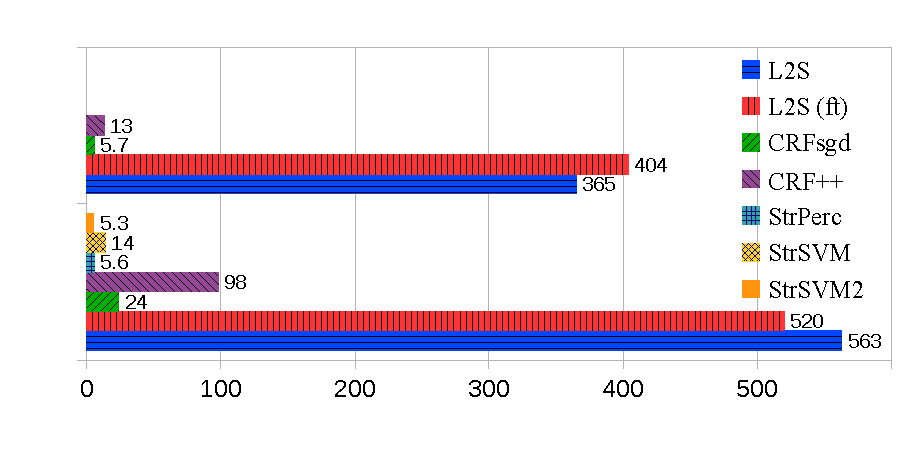
\includegraphics[scale=0.9]{tokenposec.pdf}
  \caption[Usporedba brzine označavanja metoda strukturnog
  predviđanja.]{Usporedba brzine označavanja metoda strukturnog predviđanja.
  Prikazani brojevi su u tisućama po sekundi. Slika se u izvornom obliku nalazi
  u \citep{ltsicmltutorial}.}
  \label{fig:ltsperf}
\end{figure}


\section{Opis skupa podataka za učenje i testiranje}
Podaci korišteni za vrednovanje modela zadataka koji slijede koriste univerzalan
CoNLL-U format opisan u \citep{univdeps12}, a preoblikovani su iz originalnog skupa
podataka \textsc{SETimes.HR} \citep{agic2014setimes}. Popis svih raspoloživih
jezika i poveznice za preuzimanje skupa podataka prisutan je na
\href{http://universaldependencies.org/}{universaldependencies.org}.


\section{Označavanje vrste riječi}
Za vrednovanje učinkovitosti koristi se mjera točnosti \engl{accuracy}. Za
usporedbu se koriste rezultati dobiveni u \citep{agic2013lemmatization} koji su
dobiveni HunPos označivačem. Vrednovanje se vrši na dva testna skupa
(\textsc{SETimes.HR} i \textsc{Wiki}).\footnote{Datoteke
\texttt{set.hr.test.conll} i \texttt{wiki.hr.test.conll} prisutne na poveznici
\url{https://github.com/ffnlp/sethr}} Vjerojatno su u međuvremenu postignuti
bolji rezultati od navedenih, ali nisu zabilježeni u raspoloživoj literaturi.

U tablici \ref{table:postagging} prikazani su rezultati. Uz prijašnje rezultate
prikazana je uspješnost običnog označivača vrste riječi (\textsc{Vwpos 1} --
alg.~\ref{alg:postagging}) i označivača s više prolaza (\textsc{Vwpos 2} --
alg.~\ref{alg:postagging:multipass}). Korištene značajke su prefiksi i sufiksi
do najveće duljine od pet znakova, oblik riječi u kojem su mala i velika slova
zamijenjeni slovom \textsc{l} i \textsc{u}, dvije susjedne riječi lijevo i desno
od trenutne i duljina riječi. Donošenje trenutne odluke uvjetuje se s tri prošle
odluke. U slučaju \textsc{Vwpos 2} algoritma korištena su 3 prolaza. Kod HunPos
označivača koristi se Markovljev lanac drugog stupnja, a za rezultate na
\textsc{Wiki} testnom skupu i dodatni vanjski leksikon.

\begin{table}
\centering
\caption[Rezultat označavanja vrste riječi.]{Rezultat označavanja vrste riječi.}
\label{table:postagging}
\begin{tabular}{|l|c|c|}
\hline
Metoda             & \textsc{Set}   & \textsc{Wiki}  \\ \hline \hline
HunPos             & 97.04          & 94.62          \\
\textsc{Vwpos 1}   & 98.18          & 96.20          \\
\textsc{Vwpos 2}   & \textbf{98.71} & 96.24          \\
\textsc{Vwmsd} 1   & 98.31          & \textbf{96.57} \\
\textsc{Vwmsd} 2   & 98.23          & 96.41          \\ \hline
\end{tabular}
\end{table}

U tablici \ref{table:msdtagging} prikazani su rezultati za označavanje koristeći
morfosintaktičke deskriptore. Značajke korištene identične su kao i za prethodni
zadatak. Pristupi \textsc{Vwpos 1} i \textsc{2} koriste se tako da se svaka
morfosintaktička oznaka gleda kao zasebna oznaka vrste riječi (takvih u
korištenom skupu ima 645). Pristupi \textsc{Vwmsd} 1 i 2 gledaju
morfosintaktičke odluke kao oznake vrste riječi s atributima. U svakom pristupu
za svaku riječ donosi se niz odluka koje na kraju rezultiraju potpunim ispravnim
morfosintaktičkim deskriptorom.  Kod pristupa \textsc{Vwmsd 1} trenutna odluka
uvjetovana je svim predthodnim odlukama za dvije prošle riječi i trenutnu riječ,
a za \textsc{Vwmsd 2} korištene su sve donesene odluke na prethodne dvije i
sljedeće dvije riječi.

U oba \textsc{Vwmsd} pristupa za riječ prvo odaberemo oznaku vrste riječi (jednu
od trinaest mogućih). Nakon toga moguće je odabrati prvi atribut, ali ne bilo
koji nego baš onaj koji odgovara za odabranu oznaku. To smanjuje broj binarnih
odluka koje je potrebno izvršiti. Pretpostavimo da označavamo rečenicu od deset
riječi. Kod \textsc{Vwpos 1} pristupa moramo za svaku riječ pozvati 645 binarne
odluke (\textsc{ova}) što na kraju rezultira s ukupno 6450 odluka. Zbog
ograničenja mogućih vrijednosti atributa s obzirom na izabranu oznaku vrste
riječi broj odluka bi trebao biti manji. Kod donošenja odluke na prvoj razini za
riječ možemo izabrati jednu od 13 mogućih. Nakon toga, pretpostavljajući da
oznaka ima 6 mogućih atributa (zamjenica ima toliko) i da svaki atribut ima 7
mogućih vrijednosti (padež kod imenice) onda će se za pojedinu riječ morati
pozvati $13+6 \cdot 7 = 55$ binarnih odluka, što je ukupno 550 za cijelu
rečenicu. U usporedbi sa 6450 to je puno manje, a u praksi broj odluka je još
manji iz čega slijedi da je vrijeme učenja i testiranja puno manje. U tablici
\ref{table:postagging} prikazana je uspješnost \textsc{Vwmsd} pristupa na
običnom zadatku označavanja vrste riječi. \textsc{Vwmsd} pristupi imaju bolju
generalizaciju od \textsc{Vwpos 1} pristupa, ali očito povećani broj značajki
(svaka prijašnja odluka kojom uvjetujemo trenutnu je nova značajaka) zahtijeva
više podataka za bolju generalizaciju. Moguće je da u lancu odluka koji
potreban za formiranje jednog morfosintaktičkog deskriptora dolazi lakše do
grešaka nego u slučaju da se jedan morfosintaktički deskriptor promatra kao
jedinstvena odluka. Ovaj bi slučaj upućivao na prisutnost pristranosti odlukama
koja se može dogoditi ako klasifikator nije dobro naučen. Razlog lošijim
rezultatima na testnom skupu \textsc{Wiki} je taj što skup sadrži više neviđenih
riječi i nepoznate morfosintaktičke deskriptore. Zbog toga pristupi koji donose
odluke po atributima imaju bolju generalizaciju na tom skupu. Ako se kreiraju
novi skup za treniranje i testiranje koji koriste sve rečenice iz svih skupova,
onda \textsc{Vwpos 2} ima najbolju točnost.

\begin{table}
\centering
\caption[Rezultat označavanja vrste riječi koristeći morfosintaktičke
deskriptore.]{Rezultat označavanja vrste riječi koristeći morfosintaktičke
deskriptore. Prikazana je točnost modela na dva testna skupa.}
\label{table:msdtagging}
\begin{tabular}{|l|c|c|}
\hline
Metoda             & \textsc{Set}   & \textsc{Wiki}  \\ \hline \hline
HunPos             & 87.11          & 80.83          \\
\textsc{Vwpos 1}   & 89.94          & 83.27          \\
\textsc{Vwpos 2}   & \textbf{90.22} & \textbf{84.13} \\
\textsc{Vwmsd 1}   & 89.19          & 82.22          \\
\textsc{Vwmsd 2}   & 89.06          & 81.90          \\ \hline
\end{tabular}
\end{table}


\section{Parsiranje ovisnosnih stabala}
\citep{agic2013three}.


\section{Združeno označavanje vrste riječi i parsiranje}
Koriste se iste mjere učinkovitosti za vrednovanje modela i iste značajke
opisane u prijašnjim potpoglavljima. Podatkovni skup za učenje i testiranje je
za ovaj združeni zadatak samo iz UD, a za potrebe usporedbe razdvojen je u dva
skupa koji su identični \textsc{Set} i \textsc{Wiki} u rečenicama.

\begin{table}
\centering
\caption{Rezultat označavanja vrste riječi sa združenim modelom.}
\label{table:taggingjoint}
\begin{tabular}{|l|l|l|l|l|}
\hline
Metoda             & \textsc{\textunderscript{Set}{pos}} & \textsc{\textunderscript{Wiki}{pos}} & \textsc{\textunderscript{Set}{msd}} & \textsc{\textunderscript{Wiki}{msd}} \\ \hline \hline
\textsc{Vwpos 2}   & \textbf{98.71}                      & 96.24                                & 90.22                               & 84.13                 \\
\textsc{Vwjoint 1} & 98.69                               & \textbf{97.23}                       & \textbf{92.03}                      & \textbf{85.01}        \\ \hline
\end{tabular}
\end{table}

U tablici \ref{table:taggingjoint} prikazana je učinkovitost združenog modela
samo na zadatku označavanja vrste riječi. Za usporedbu je prikazan najuspješniji
model na tom zadatku \textsc{Vwpos 2}. Očito nije lako unaprijediti označavanje
osnovnih oznaka vrste riječi, ali se vidi bitan skok u učinkovitosti kod
morfosintaktičkih deskriptora -- UD ne koristi sve atribute koje ima
\textsc{SETimes.HR}, ali učinkovitost bez tih atributa nije značajno
promijenjena. Skok je bio očekivan jer postoje neki atributi koje možemo jasnije
označiti ako nam je dana informacija o sintaksi. Kako u okviru združenog učenja
dolazi do propagacije informacije o grešci nakon ovisnosnog parsiranja, onda će
zadatak označavanja vrste riječi prilagoditi svoje težine tako da izvršavanje
ovisnosnog parsiranja bude točnije. Rezultati u tablici
\ref{table:depparsing:joint} potvrđuju da združeno učenje može poboljšati
rezultate na zadatku iskorištavanjem funkcije gubitka koja u ovom slučaju daje
bolju procjenu greške. Moguće je prvo trenirati samo na jednom zadatku u
kaskadi, a onda na oba u slučaju da za prvi zadatak postoji više podataka. U
prvotnom slučaju funkcija gubitka daje lošu procjenu prave greške (jer se
združeni zadatak ne izvršava), a u naknadnom učenju cilj je pretrenirani model
prilagoditi da ima dobre performanse na združenom zadatku.

\begin{table}
\centering
\caption{Rezultat ovisnosnog parsiranja združenog modela.}
\label{table:depparsing:joint}
\begin{tabular}{|l|c|c|}
\hline
Metoda                 & \textsc{las}   & \textsc{uas}    \\ \hline \hline
\textsc{Vwdep}   (MSD) & 79.22          & 86.44           \\
\textsc{Vwjoint} (POS) & 75.44          & 83.91           \\
\textsc{Vwjoint} (MSD) & \textbf{81.01} & \textbf{88.02}  \\ \hline
\end{tabular}
\end{table}


%% -----------------------------------------------------------------------------
\chapter{Zaključak}
U okviru ovog diplomskog rada razvijeni su i vrednovani označivači vrste riječi
i ovisnosni parseri s razinama točnosti koje su usporedive s najboljim
rezultatima za hrvatski jezik koji su prisutni u literaturi. Najbolji model
postignut je koristeći združeno učenje i predviđanje na oba zadatka.


\bibliography{literatura}
\bibliographystyle{fer}
\begin{appendix}\
\lstset{literate={ć}{{\'{c}}}1}

%% TODO dodati linkove na implementaciju
\chapter{Označivači vrste riječi}
\section{Običan označivač vrste riječi}
\label{appendix:postagging}
\begin{lstlisting}[language=C++,
                   basicstyle=\tiny\ttfamily]{Name=msd-one-by-one}
void run(Search::search& sch, vector<example*>& ec)
{ Search::predictor P(sch, (ptag)0);
  for (size_t i=0; i<ec.size(); i++)
  { action oracle     = ec[i]->l.multi.label;
    size_t prediction = P.set_tag((ptag)i+1)
                         .set_input(*ec[i])
                         .set_oracle(oracle)
                         .set_condition_range((ptag)i, sch.get_history_length(), 'p')
                         .predict();

    if (sch.output().good())
      sch.output() << sch.pretty_label((uint32_t)prediction) << ' ';
  }
}
\end{lstlisting}
\newpage
\section{MSD slijedni označivač po atributima}\label{appendix:msdattr}
\begin{lstlisting}[language=C++,
                   basicstyle=\tiny\ttfamily]{Name=msd-one-by-one}
void run(Search::search& sch, vector<example*>& ec)
{ Search::predictor P(sch, (ptag)0);
 task_data * data = sch.get_task_data<task_data>();
 resize_tags(data, ec.size());
 size_t pass = 0, shift = 1;
 for (size_t i=0; i<ec.size(); i++)
 {
   while (has_positional_decision(data, i, pass)) {
     ptag p = (ptag)shift;
     action oracle     = get_label(ec[i], pass);
     v_array<action> & allowed = get_allowed(data, pass, i);
     P.set_tag(p).set_input(*ec[i]).set_oracle(oracle).set_allowed(allowed);

     if (i > 0) {
       size_t start = i < sch.get_history_length() ? 0 : i - sch.get_history_length();
       char name = 'a', prevn='a'; // for erasing previous conditions
       for(size_t j = start; j < i; ++j) {
         for(tag & t : get_tags(data, j)) {
           if (name == 'a') P.set_condition(t.i, name++);
           else             P.add_condition(t.i, name++);
         }
         name = prevn + 10; prevn = name;
       }
     }

     size_t prediction = P.predict();
     push_tag(data, i, p, prediction, pass);

     sch.loss(prediction != oracle);
     if (sch.output().good()){
       sch.output() << sch.pretty_label((uint32_t)prediction);
       if (has_positional_decision(data, i, pass+1)) {sch.output() << ' ';}
       else                                          {sch.output() << '\n';}
     }
     shift += 1;
     pass += 1;
   }
   pass = 0;
 }
}
\end{lstlisting}
\newpage
\section{MSD označivač po slojevima}\label{appendix:msdlayered}
\begin{lstlisting}[language=C++,
                   basicstyle=\tiny\ttfamily]{Name=msd-one-by-one}
void run(Search::search& sch, vector<example*>& ec)
{ Search::predictor P(sch, (ptag)0);
  task_data * data = sch.get_task_data<task_data>();
  resize_tags(data, ec.size());
  size_t pass = 0, shift = 1; bool touched = true;
  while (touched) {
    touched = false;
    for (size_t i=0; i<ec.size(); i++)
    { if (has_positional_decision(data, i, pass)) {
        ptag p = (ptag)shift;
        action oracle     = get_label(ec[i], pass);
        v_array<action> & allowed = get_allowed(data, pass, i);
        P.set_tag(p).set_input(*ec[i]).set_oracle(oracle).set_allowed(allowed);

        size_t start = i < sch.get_history_length() ? 0 : i - sch.get_history_length()/2;
        size_t end = pass == 0 ? i : std::min(i+1 + sch.get_history_length()/2, ec.size());
        char name = 'a', prevn = 'a'; // for erasing previous conditions
        for(size_t j = start; j < end; ++j) {
          if (j == i) continue;
          for(tag & t : get_tags(data, j)) {
            if (name == 'a') P.set_condition(t.i, name++);
            else             P.add_condition(t.i, name++);
          }
          name = prevn + 10; prevn = name; // no msd has more than 10 labels
        }
        size_t prediction = P.predict(); push_tag(data, i, p, prediction, pass);
        shift += 1; touched = true;
      }
    }
    pass += 1;
  }
  int loss = 0;
  for(int j = 0; j < ec.size(); ++j){
    pass = 0;
    for(tag & t : get_tags(data, j)) {
      if (t.a !=  get_label(ec[j], pass++)) {
        loss += 1; break;
      }
    }
  }
  sch.loss(loss);
  if (sch.output().good()){
    for(int j = 0; j < ec.size(); ++j){
      pass = 0;
      for(tag & t : get_tags(data, j)) {
        sch.output() << sch.pretty_label((uint32_t)t.a);
        if (has_positional_decision(data, j, ++pass)) {sch.output() << ' ';}
        else                                          {sch.output() << '\n';}
      }
    }
  }
}
\end{lstlisting}

\chapter{Podaci}\label{appendix:data}
\section{SETimes.HR}
\begin{lstlisting}[basicstyle=\tiny\ttfamily]
1       Proces  proces  N       Ncmsn   Type=common|Gender=masculine|Number=singular|Case=nominative    0       Elp     6:nsubj UposTag=NOUN|Case=Nom|Gender=Masc|Number=Sing
2       privatizacije   privatizacija   N       Ncfsg   Type=common|Gender=feminine|Number=singular|Case=genitive       1       Obj     1:nmod  UposTag=NOUN|Case=Gen|Gender=Fem|Number=Sing
3       na      na      S       Sl      Case=locative   1       Prep    4:case  UposTag=ADP|Case=Loc
4       Kosovu  Kosovo  N       Npnsl   Type=proper|Gender=neuter|Number=singular|Case=locative 3       Adv     6:nmod  UposTag=PROPN|Case=Loc|Gender=Neut|Number=Sing
5       pod     pod     S       Si      Case=instrumental       0       Prep    6:case  UposTag=ADP|Case=Ins
6       povećalom       povećalo        N       Ncnsi   Type=common|Gender=neuter|Number=singular|Case=instrumental     5       Elp     0:root  UposTag=NOUN|Case=Ins|Gender=Neut|Number=Sing
\end{lstlisting}

\section{UD}
\begin{lstlisting}[basicstyle=\tiny\ttfamily]
1       Proces  proces  NOUN    _       Case=Nom|Gender=Masc|Number=Sing        6       nsubj   _       _
2       privatizacije   privatizacija   NOUN    _       Case=Gen|Gender=Fem|Number=Sing 1       nmod    _       _
3       na      na      ADP     _       Case=Loc        4       case    _       _
4       Kosovu  Kosovo  PROPN   _       Case=Loc|Gender=Neut|Number=Sing        6       nmod    _       _
5       pod     pod     ADP     _       Case=Ins        6       case    _       _
6       povećalom       povećalo        NOUN    _       Case=Ins|Gender=Neut|Number=Sing        0       root    _       _
\end{lstlisting}

\section{\textsc{vw} - označavanje vrste riječi}
\begin{lstlisting}[basicstyle=\tiny\ttfamily]
2 |w Proces proces 0:6 ulllll
2 |w privatizacije privatizacije 0:13 lllllllllllll
1 |w na na 0:2 ll
2 |w Kosovu kosovu 0:6 ulllll
1 |w pod pod 0:3 lll
2 |w povećalom povećalom 0:9 lllllllll
\end{lstlisting}
\section{\textsc{vw} - ovisnosno parsanje}
\begin{lstlisting}[basicstyle=\tiny\ttfamily]
6 1 |w Proces |p NOUN  NOUNCase=Nom NOUNGender=Masc NOUNNumber=Sing
1 2 |w privatizacije |p NOUN  NOUNCase=Gen NOUNGender=Fem NOUNNumber=Sing
4 3 |w na |p ADP  ADPCase=Loc
6 2 |w Kosovu |p PROPN  PROPNCase=Loc PROPNGender=Neut PROPNNumber=Sing
6 3 |w pod |p ADP  ADPCase=Ins
0 4 |w povećalom |p NOUN  NOUNCase=Ins NOUNGender=Neut NOUNNumber=Sing
\end{lstlisting}

\chapter{Analiza sentimenta}\label{appendix:sentiment}
\section{Prvo dokument onda rečenice}
\begin{lstlisting}[language=C++,
                   basicstyle=\tiny\ttfamily]{Name=msd-one-by-one}
void run(Search::search& sch, vector<example*>& ec)
{ Search::predictor P(sch, (ptag)0);
  action oracle = ec[0]->l.multi.label;
  size_t global_prediction = P.set_tag(1 /* global tag */).set_input(*ec[0]).set_oracle(oracle).predict();
  if (sch.output().good())
      sch.output() << sch.pretty_label((uint32_t)global_prediction) << ' ';
  for (size_t i=1; i<ec.size(); i++)
  { oracle     = ec[i]->l.multi.label;
    size_t prediction = P.set_tag((ptag)i+1)
                         .set_input(*ec[i])
                         .set_oracle(oracle)
                         .set_condition_range((ptag)i, sch.get_history_length(), 'p')
                         .add_condition(1 /* global tag */, 'a') // adds the global as condition on each sequence element
                         .predict();

    if (sch.output().good())
      sch.output() << sch.pretty_label((uint32_t)prediction) << ' ';
  }
}
\end{lstlisting}
\section{Prvo rečenice onda dokument}
\begin{lstlisting}[language=C++,
                   basicstyle=\tiny\ttfamily]{Name=msd-one-by-one}
void run(Search::search& sch, vector<example*>& ec)
{ Search::predictor P(sch, (ptag)0);
  for (size_t i=0; i<ec.size()-1; i++)
  { action oracle     = ec[i]->l.multi.label;
    size_t prediction = P.set_tag((ptag)i+1)
                         .set_input(*ec[i])
                         .set_oracle(oracle)
                         .set_condition_range((ptag)i, sch.get_history_length(), 'p')
                         .predict();

    if (sch.output().good())
      sch.output() << sch.pretty_label((uint32_t)prediction) << ' ';
  }
  action oracle = ec.back()->l.multi.label;
  size_t global_prediction = P.set_tag(ec.size())
                              .set_input(*ec.back())
                              .set_oracle(oracle)
                              .set_condition_range(ec.size()-1, ec.size()-1, 'a').predict();
                              // conditioning on all previous sequence decisions
  if (sch.output().good())
      sch.output() << sch.pretty_label((uint32_t)global_prediction) << ' ';
}
\end{lstlisting}
\end{appendix}


\begin{sazetak}
Sažetak na hrvatskom jeziku.

\kljucnerijeci{učenje pretraživanja, obrada prirodnog jezika, strojno učenje}
\end{sazetak}


\engtitle{Learning to search for natural language processing problems}
\begin{abstract}
Abstract.

\keywords{learning to search, natural language processing}
\end{abstract}


\nocite{daume06thesis}
\nocite{daume09searn}
\nocite{daume06searn-practice}
\nocite{daume15reductions}
\nocite{daume15lols}
\nocite{daume14lts}

\end{document}
